\chapter{The Forward Tagger}

\section{The MesonEx Program}

\subsection{The MesonEx Program}
Meson spectroscopy
Quark model describes baryons and mesons as bound states of 3 quarks and a quark anti-quark pair. Desbribes well many of the features of the hadron spectrum. However recent developments have shown that the hadron mass cannot simply me describes in terms of the masses of the constituent quarks, but it mainly due to the dynamics of the interacting gluons that bind the system together. The simpler 2 or 3 quark bound state desciptions is a simplification of the much more complex ever evolving quark-gluon plasma present in all hadrons. Studying the spectrum of hadrons and measuring the properties to learn more about their inner stucture is crucial in developing a deeper understanding of the mechanics of the strong nuclear force.


\textbf{Notes for the rest of the section} 

Mesons, composed of a quark and a anti-quark pair, are the simplest bound quark state and form an ideal environment to study the interactions within hadrons. 
Study confinement.
The role gluons play in QCD.
Quark model predicts the existence of multiplets of mesons with differentiated by the properties of total angular momentum J, parity P and charge conjugation C.
Most of the lowest mass states have been identified and studied.
Some issues still remain.
Models of QCD and lattice calculations predict that states beyond a simple $q\bar{q}$ configuration such as tetraquarks$(qq\bar{q}\bar{q})$, hybrids (qqg)and glueballs, should also exist.
If this is the case we should expect to see a much richer and varied spectrum of hadronic states than is predicted by the quark model.

\subsection{Electroproduction at very small $Q^2$}
%At 11 GeV/c the previous method of producing real bremsstrahlung photons tagged by a magnetic calorimeter is no longer possible due to the limitations of the existing magnet. Instead the plan is to use quasi-real photons produced when electrons are scattered at very small angles (low $Q^2$). This technique has been previously used 


\section{The Forward Tagger}
A new detector system designed to measure particle properties at forward angles, between 2 and 4.5 degrees from the beamline. It has been designed to optimally detect the properties of electrons scattered at very small angles with an acceptance exceeding $99\%$. \cite{FTTDR2012} The new detector will be placed between the High Threshold Cherenkov Counter (HTCC) and the torus suppport within CLAS, in a limited space at most $\sim$ 40 cm in length, just under 2m downsteam of the (nominal) target position. The detector is composed of three major sub-systems:

\begin{itemize}
	\item	Electromagnetic Calorimeter (FT-Cal)
	\item   Scintillation Counter (FT-Hodo)
	\item   Tracker (FT-Trck)
\end{itemize}

The FT-Cal will detect the electrons, measure the energy of the electromagnetic shower and provide a fast trigger for other detector systems in CLAS. The FT-Trck will measure the scattering angles ($\theta_{e}$ and $\phi_{e}$). The FT-Hodo provides e/$\gamma$ separation and further background reduction by taking measurements in coincidence with the calorimeter.

The limited region available for the detector and the close proximity to the beamline (2.5\textdegree coresponds to $\sim$ 8 cm) necessitates compact detector systems that are able to process the very high flux present while remaining highly resistant to radiation damage. All components are contained with a region \textless5\textdegree from the beamline, to minimize interfere with any of the other systems in CLAS. 

A brief overview of the main subsystems of the detector will be given in the following section before going to explore in more depth the design of the FT-Hodo which is the main focus of this thesis.

\begin{figure}
	\centering
	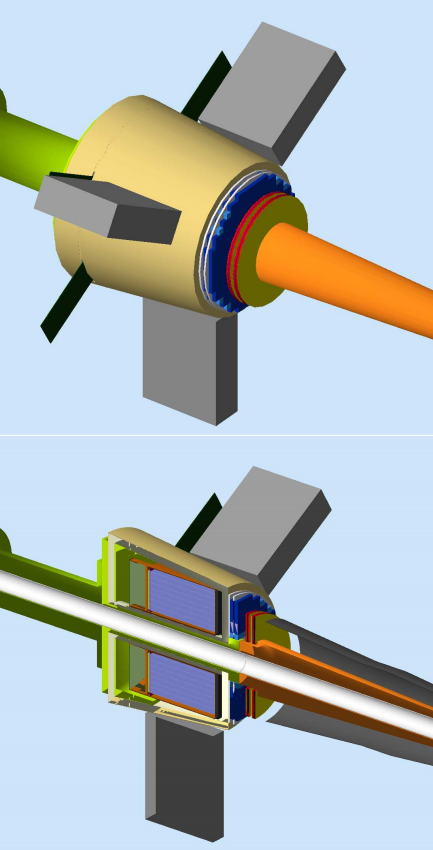
\includegraphics[width=0.6\textwidth]{ImgChap1/FTcross}
	\caption{Cross section of the forward tagger. \cite{FTTDR2012} }
	\label{FTcross}
\end{figure}



%Give some background and context to the work.
%Define the relevence of the area and why there is interesting work to be done there.
%Give some context of the current state of research and where JLAB fits into this.
%Discuss about CLAS, then about CLAS12, then about the forward tagger.
%Go on to discuss the purpose of the hodoscope and overall design contraints.
%General overview of the design key elements of interest.
%Discuss the key decision areas in detail. Tiles, Fibres, SiPMs, Reflective materials etc.
%Discuss the ongoing testing and literature research that lead to the decisions made.

\subsubsection{FT-Cal}
The FT-Cal is a highly segmented lead tungstate based electromagnetic calorimeter that has to fulfil demanding requirements in a limited space. The detector requires, high light yield and a fast recovery time ($\sim$ 10 ns) for high energy resolution and minimal pile up within the detector. Excellent timing resolution for tagger events in conjunction with other systems within CLAS. Finally it requires high radiation hardness, combined with a small radiation length and Moliere radius within the detector.

To achieve these objectives the detector was designed to be highly segmented in the transverse direction to maintain a sustainable output rate from each pixel. In addition the traverse size of each element should be comparable to the typical Moliere radius of the electromagnetic shower produced in the detector. This will minimise unnecessary pixel firing by containing the shower to a limited number of crystals. A simple diagram of the FT-Cal is shown in Figure \ref{ftcalo} with the showing the arrangement of the crystals.

\begin{figure}
	\centering
	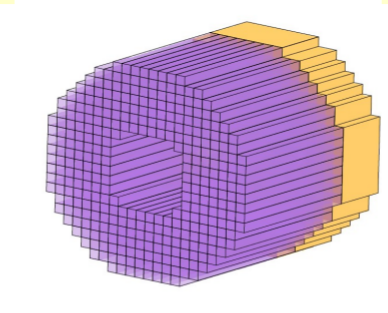
\includegraphics[width=0.6\textwidth]{ImgChap1/ftcalo}
	\caption{A simple schematic of the geometry of the forward tagger calorimeter. With each of the individual lead tungstate crystals highlighted in purple and the readout systems in yellow. \cite{FTTDR2012}}
	\label{ftcalo}
\end{figure}


Lead tungstate ($PbWO_{4}$) has been extensively studied and used in several large scale detectors in recent years. \cite{zhou2007phos,erni2008technical}It was selected for crystals due to its fast scintillation decay time (6.5 ns), a small radiation length (0.9 cm), and limited Moliere radii (2.1 cm). The main disadvantage of the material is its limited light yield ($0.3\%$ of NaI(TI)). However recent improvements to manufacturing processes and cooling of the material below 0\textdegree{C} has shown an improvement in this by a factor of 6-8. With this configuration an energy resolution of $2\% / \sqrt{E(GeV)} \oplus 1\%$ is expected. \textbf{Need to understand this better} \cite{FTTDR2012}

The readout from the detector is required to operate in a high magnetic field excluding standard photomultiplers. Instead Avalanche Photo Diodes (APD) were selected as they have been shown to be both radiation hard and perform well under such conditions. Further information on the design and properties of the FT-Cal can be found in the forward tagger technical design report. \cite{FTTDR2012}.


\subsubsection{FT-Hodo}

The main design objective of the hodoscope is to differentiate between photons and electrons in the calorimeter. The two particles produce indistinguishable electromagnetic showers in the FT-Cal and additional information from the scintiallator tiles in the hodoscope is required. Electrons will be identified by observing near simultaneous hits correlated in both position and time in the FT-Hodo and FT-Cal. To achieve this objective the FT-Hodo must provide highly efficient charged particle detection with similar spacial and timing resolutions to the calorimeter.

The forward tagger comprises a two layered array of fast response plastic scintillator tiles, a thicker layer for improved timing resolution and a thin layer for enhanced background rejection. The positioning of the detector elements in the hodoscope will mirror the layout of the FT-Cal, ensuring uniform coverage across the two detector systems. The restrictive geometry of the volume occupied by the forward tagger precludes the use of standard light guides and photomultipliers. Instead each element is read out using embedded wavelength shifting fibres (WLS) which are flexible and enhance the performance of the readout silicon photomultipliers (SiPM). Similar systems have been used in the past to achieve the sub ns timing resolution required \cite{stepanyan2008clas}. Figure \ref{fthodo} shows a simplistic depiction of the hodoscope in relation to the calorimeter.

\begin{figure}
	\centering
	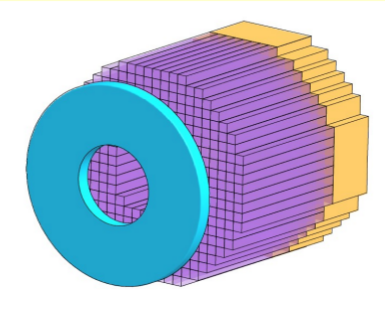
\includegraphics[width=0.6\textwidth]{ImgChap1/fthodo}
	\caption{A simplistic representation of the hodscope, highlighted in light blue, is shown in relation to the calorimeter. \cite{FTTDR2012} }
	\label{fthodo}
\end{figure}

The vast majority of particles incident on the hodoscope will be highly relativistic leaving a fixed minimum ionising deposition in the detector regardless of particle type. As a result having high energy resolution for the energy deposited in each elements is not critical for the detector performance. The main requirements for high detection efficiency and high timing resolution are the number of photons that reach the SiPMs and the efficiency of these detectors to convert these into measurable signals.

%Designed to discriminate between and electrons and photons arriving at the forward tagger with sub nano-second timing accuracy.
%Segmented design composed of two laters of fast responce plastic scintillators coupled by wavelength shifting fibres to Silicon photomultipliers.
%Works in conjuction with the calorimeter and tracker to provide accurate tagging information.
\subsubsection{FT-TrcK}

The role of the FT-Trck is to provide precision positional information to reconstruct the vertex angles of particles entering the forward tagger. It is composed of two doubled layers micromegas detectors with a spatial resolution of $\pm 200\mu{m}$. Each will provide an independent measurement of the (X,Y) co-ordinates and act in conjunction with hits in the hodoscope and calorimeter to improve background rejection. Figure \ref{fttrck} shows the position of the FT-Trck in relation to the FT-Cal and FT-Hodo.

\begin{figure}
	\centering
	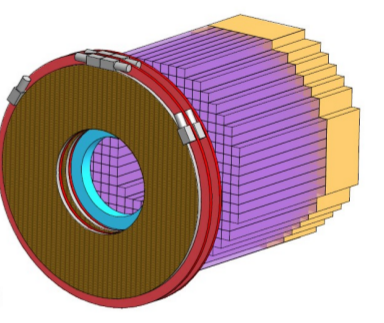
\includegraphics[width=0.6\textwidth]{ImgChap1/fttrck}
	\caption{The three major subsystems of the forward tagger are shown with the FT-trck, highlighted in brown and red, superimposed in front of the FT-Hodo and FT-Cal. \cite{FTTDR2012} }
	\label{fttrck}
\end{figure}

This configuration of the FT-Trck is expected to achieve angular resolutions of $\sim$ 1.7$\%$ and 2.8\textdegree in $\theta$ and $\phi$ respectively.
Further information on the design and properties of the FT-Cal can be found in the forward tagger technical design report. \cite{FTTDR2012}.



\section{Design of the Hodoscope}

This section will discuss in more detail the design of the hodoscope based on the contraints and aims of its construction. Critical points will be highlighted and the interconnected nature of different elements elaborated upon. However deeper discussion into the developmental decisions made and their consequences in the operation of the hodoscope are reserved for Chapter \textbf{TBC} where important sub-systems will be covered in more depth.

As discussed in the previous section the main requirement of the hodoscope is to differentiate between electrons and photons hits in the calorimeter which produce nearly indistinguishable electromagnetic showers. Whilst minimising photon misidentification and suppress false events created through photon conversion. As discussed in \textbf{section SOMETHING} this required a two layered design. The design aims to achieve this with sub-nanosecond timing resolution, to function as part of the trigger system and to not compromise the timing of the calorimeter. It will achieve $>99\%$ particle detection efficiency for the lifetime of its use and achieve this under conditions of high radiation flux and 5T magnetic fields.


The hodoscope is positioned upstream of the FT-Cal fitting within the volume of a circular disk, no more than, 330mm in diameter and 40mm depth. This limited space and harsh operating environment required an innovative approach to its development to optimise the performance of the detector system. However the initial design from which the evolution of the detector design developed is based on proven and tested detector systems. \textbf{Some discussion of literature here?}


Here are general papers on similar detectors.
\cite{reiche2001studies}
\cite{wojcik1994embedded}
\cite{cohn1993scintillating}
\cite{budd2001cms}
\cite{artikov2006new}
\cite{albrow1987uranium}
\cite{barsuk2000fiber}
\cite{adloff2010construction}

The design of the FT-Hodo is based around a segmented array of plastic scintillator tiles (EJ-204) embedded with Wavelength shifting (WLS) fibres (Kuraray Y-11) and read out by 3x3mm Silicon Photomultipliers (SiPM) (Hamamatsu S13360-3075PE). 


\subsection{Plastic Scintillator Tiles}
The plastic scintillators provide fast timing, sufficient light yield and resistance to radiation necessary in the high flux environment of the forward tagger. The limited space, radiation and magnetic fields present in the detector volume required signals to be read out externally. WLS fibres were selected for their flexibility, excellent optical characteristics and radiation resistance. These fibres shift the wavelength of light outputted by the scintillators into the ideal operation range for the SiPMs, however their attenuation length is relatively short at \textbf{<3.5m Check this}. Due to the geometry of CLAS and the enviroment whilst the beam is active the light needs to be transported more than 5m to reach the SiPMs. To resolve this after $\sim$ 10cm, still within the volume of the detector, the WLS fibres are fusion spliced to clear optical fibres which have an attenuation length \textbf{>10m Check this}. This combination allows the scintillation photons to be transported to the readout SiPMs with a light loss of less than $<40\%$. \cite{FTTDR2012}

Each layer of the forward tagger is comprised of 44 15x15mm (P15) and 72 30x30mm (P30) plastic scintillator tiles arranged with 4 fold symmetry about the axis of the beam, covering the same acceptance as the FT-Cal, shown in Figure \ref{hodotilelayout}. At the centre, nearest the beamline, there is a continuous ring of P15 tiles where the flux is expected to be at its highest. Outside this the majority of tiles are P30 type, with each one covering the same area as 4 crystals in the calorimeter. This configuration provides greater resolution in the area of greatest flux while increasing acceptance throughout the rest of the detector. 

\begin{figure}
	\centering
	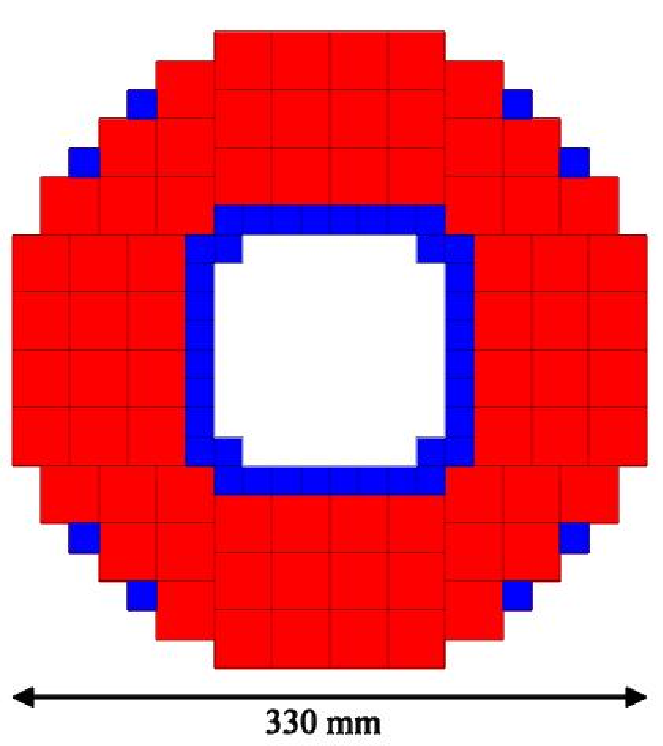
\includegraphics[width=0.6\textwidth]{ImgChap1/hodo}
	\caption{Layout of the plastic scintillator tiles in the hodoscope. 15x15mm elements are shown in blue with 30x30mm elements in red. \cite{FTTDR2012}}
	\label{hodotilelayout}
\end{figure}


\subsection{Wavelength Shifting Fibres}

The photons produced in each of the 116 tiles in each layer of the forward tagger are read out using embedded WLS fibres. These fibres absorb the typically $\sim 400nm$, photons produced in the scintillator tiles and re-emit them in green, $\sim 470nm$ optical range. The ideal operating range for the SiPMs. Each tile has diagonally drilled channels just larger than the 1mm diameter of the fibres, 4 for a P30 tile and 2 for a P15. The channels are aligned to maximise the area fibre length inside each tile, increasing the photon capture cross-section. They also allow for the fibres to feed out naturally from each tile, while maintaining close to complete acceptance of the detector system.  Figure \ref{diagonalholes} shows a photograph of a P30 tile, where the channels can be clearly observed along with the passing of the fibres out from the element.

\begin{figure}
	\centering
	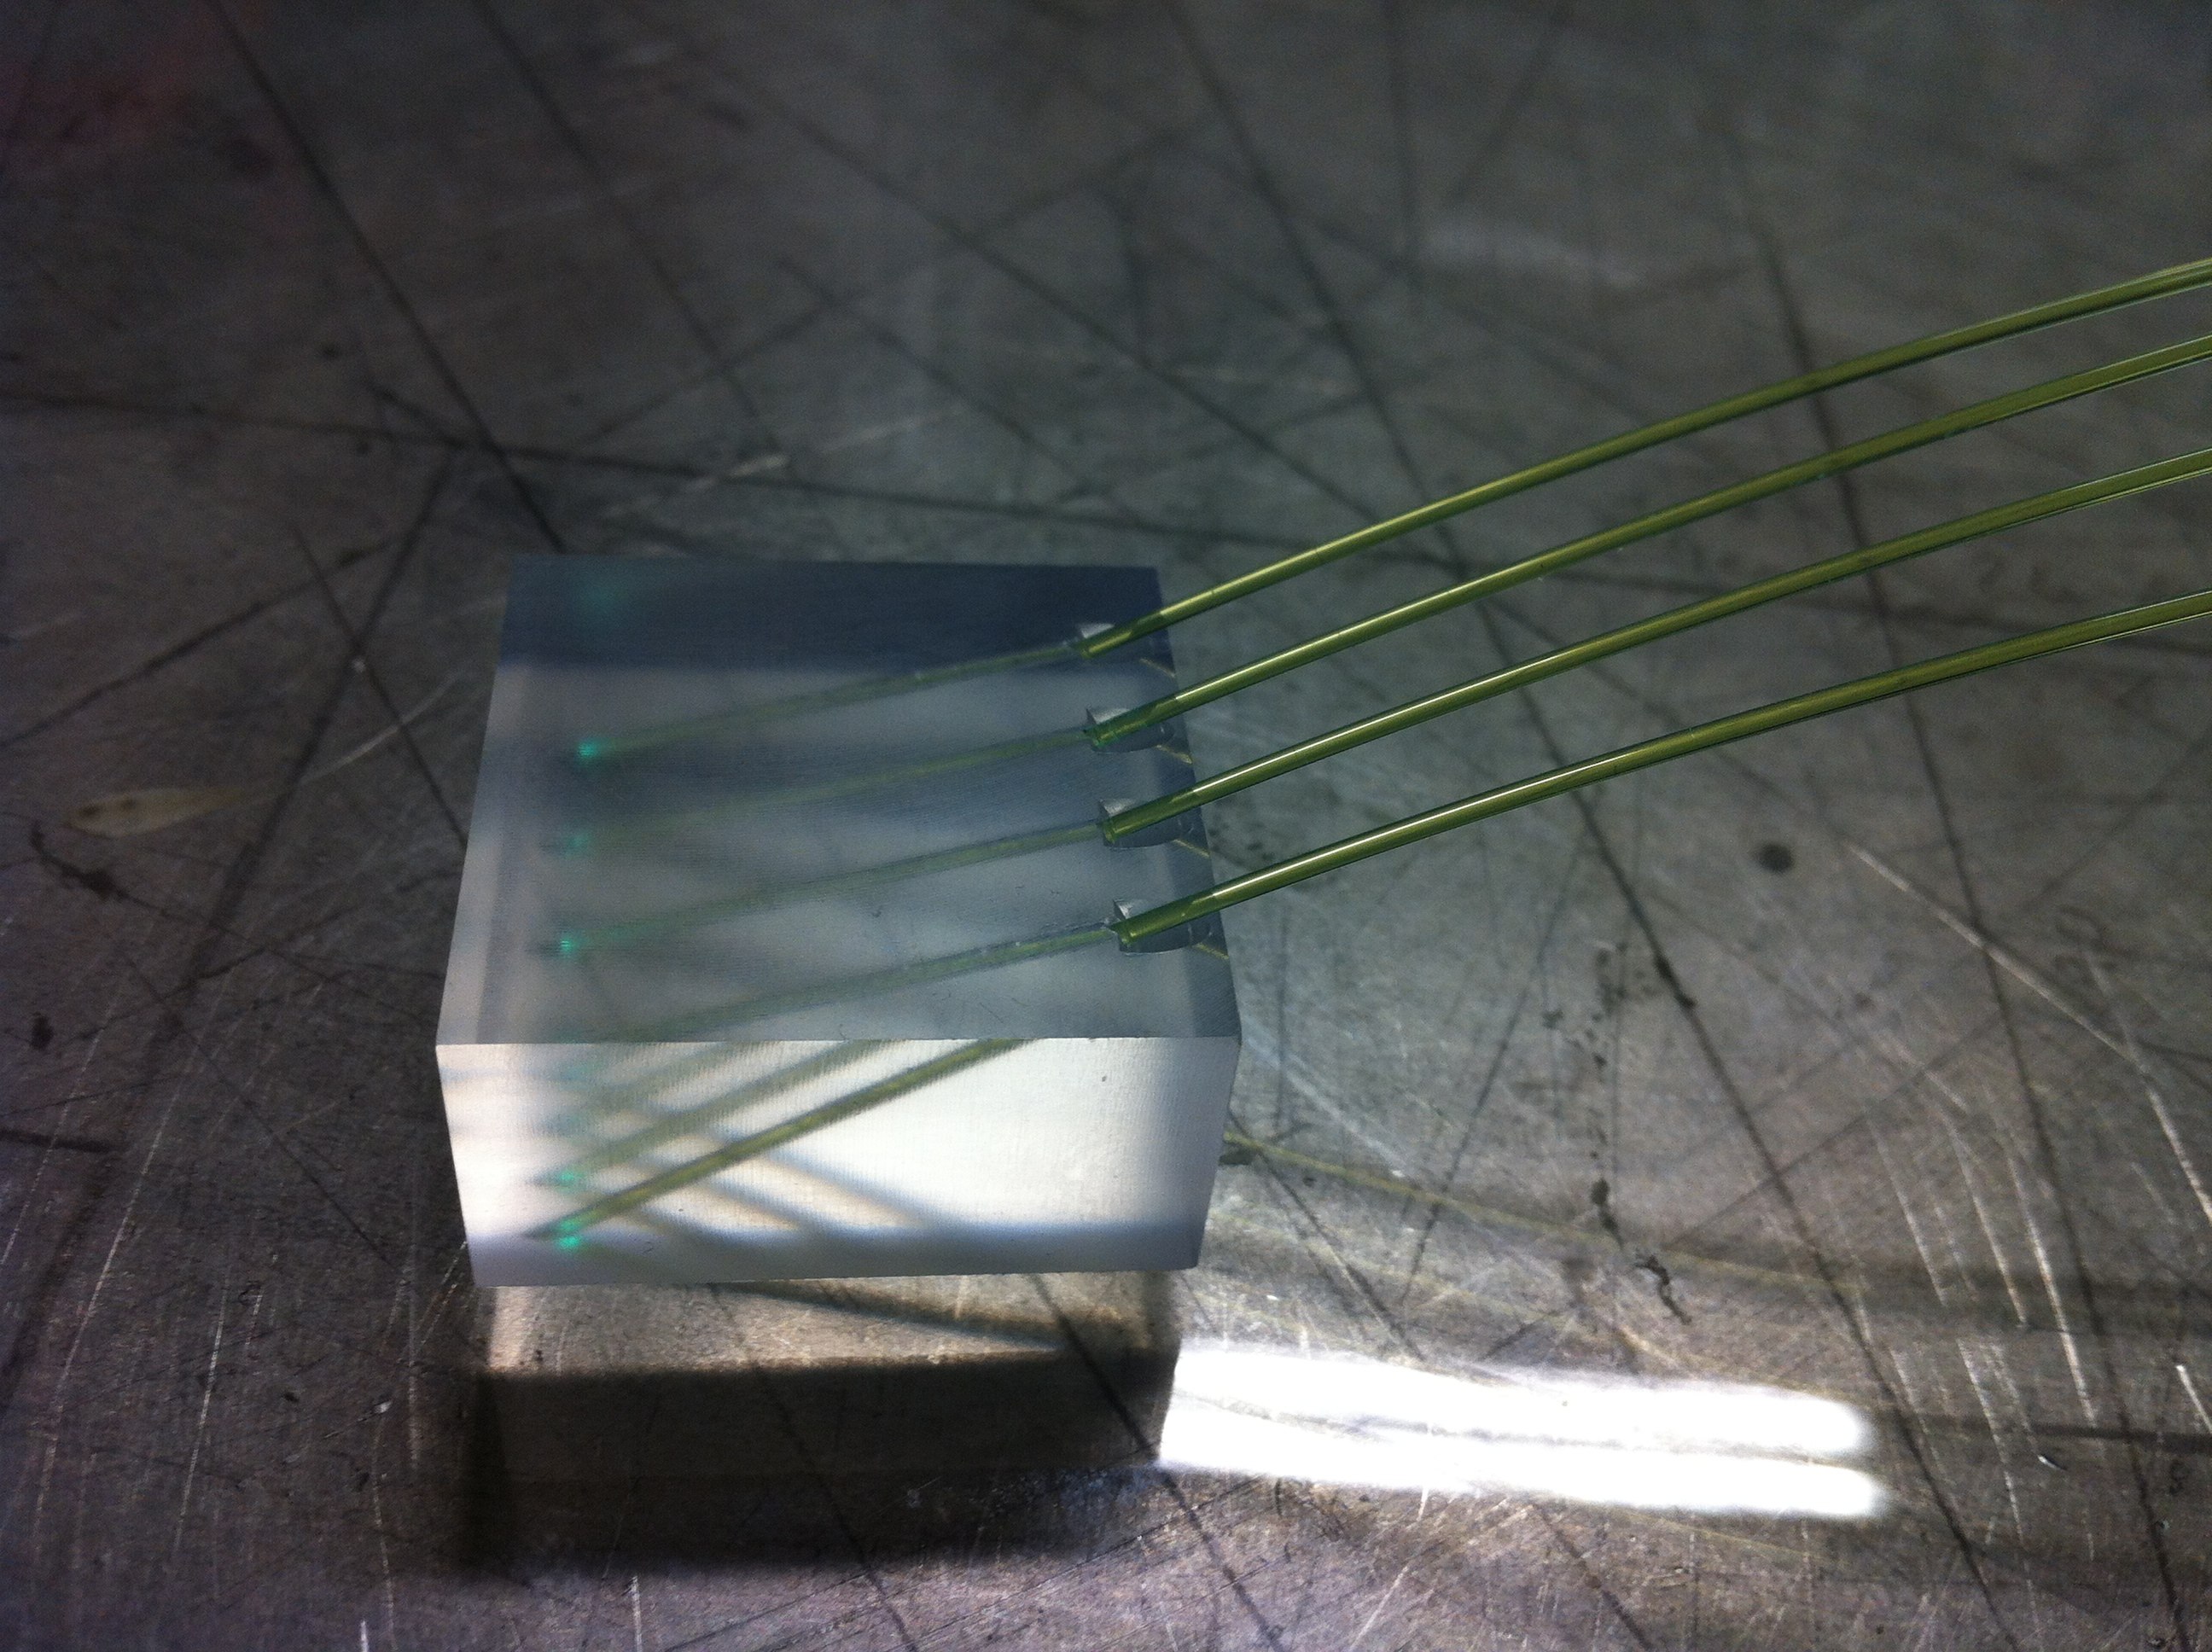
\includegraphics[width=0.6\textwidth]{ImgChap1/diagonalholes}
	\caption{A photograph of an unprepared 15mm thick p30 tiles occupied with 4 wavelength shifting fibres. The diagonally drilled channels for each fibre can be clearly seen.}
	\label{diagonalholes}
\end{figure}

The WLS fibres used in the detector are Multiclad Kuraray Y-11(200) S-Type fibres 1mm in diameter. This type of fibre has shown consistently excellent performance accross a wide array of academic studies. \textbf{need to put in the fibre references here}. The multiclad fibres produce significantly higher lightyield than traditional singleclad fibres as the two layers of differing refractive index outside the core have a much greater photon trapping efficiency. The S-Type fibres were selected for their significantly increased resistance to crasing and transmittance at smalling bending diameters ($<40mm$). This comes at the cost of transparency, leading to a $\sim 10\%$ reduction in attenuation length. Insignificant to the short lengths of WLS fibre used in the detector.

\begin{figure}
	\centering
	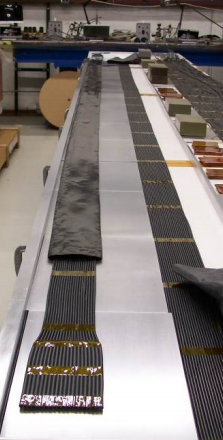
\includegraphics[width=0.5\textwidth]{ImgChap1/fibrelength}
	\caption{A photograph of the full length spliced fibres, put into groups of 4 and placed into protective black PVC sheething.}
	\label{Longfibres}
\end{figure}

The WLS fibres inserted into the tiles are fixed into place using radiation hard optical cement of similar refractive index to the scintillator and fibre. This approach minimises the photon loss across the transition and holds the fibre in place in any orientation of the hodoscope. After 10 cm each WLS fibre is fusion spliced to $\sim 5m $ long section of kuraray doubleclad clear plastic fibre, with again minimal loss of light but now transporting the photons through fibre with much greater attentuation length. This process was carried out at Fermi National Laboratory, with 10cm lengths of WLS fibre spliced to 6m lengths of clear fibre. A photograph of the sliced fibres laid out on laboratory benches is shown in Figure \ref{Longfibres}. 
  
\begin{figure}
	\centering
	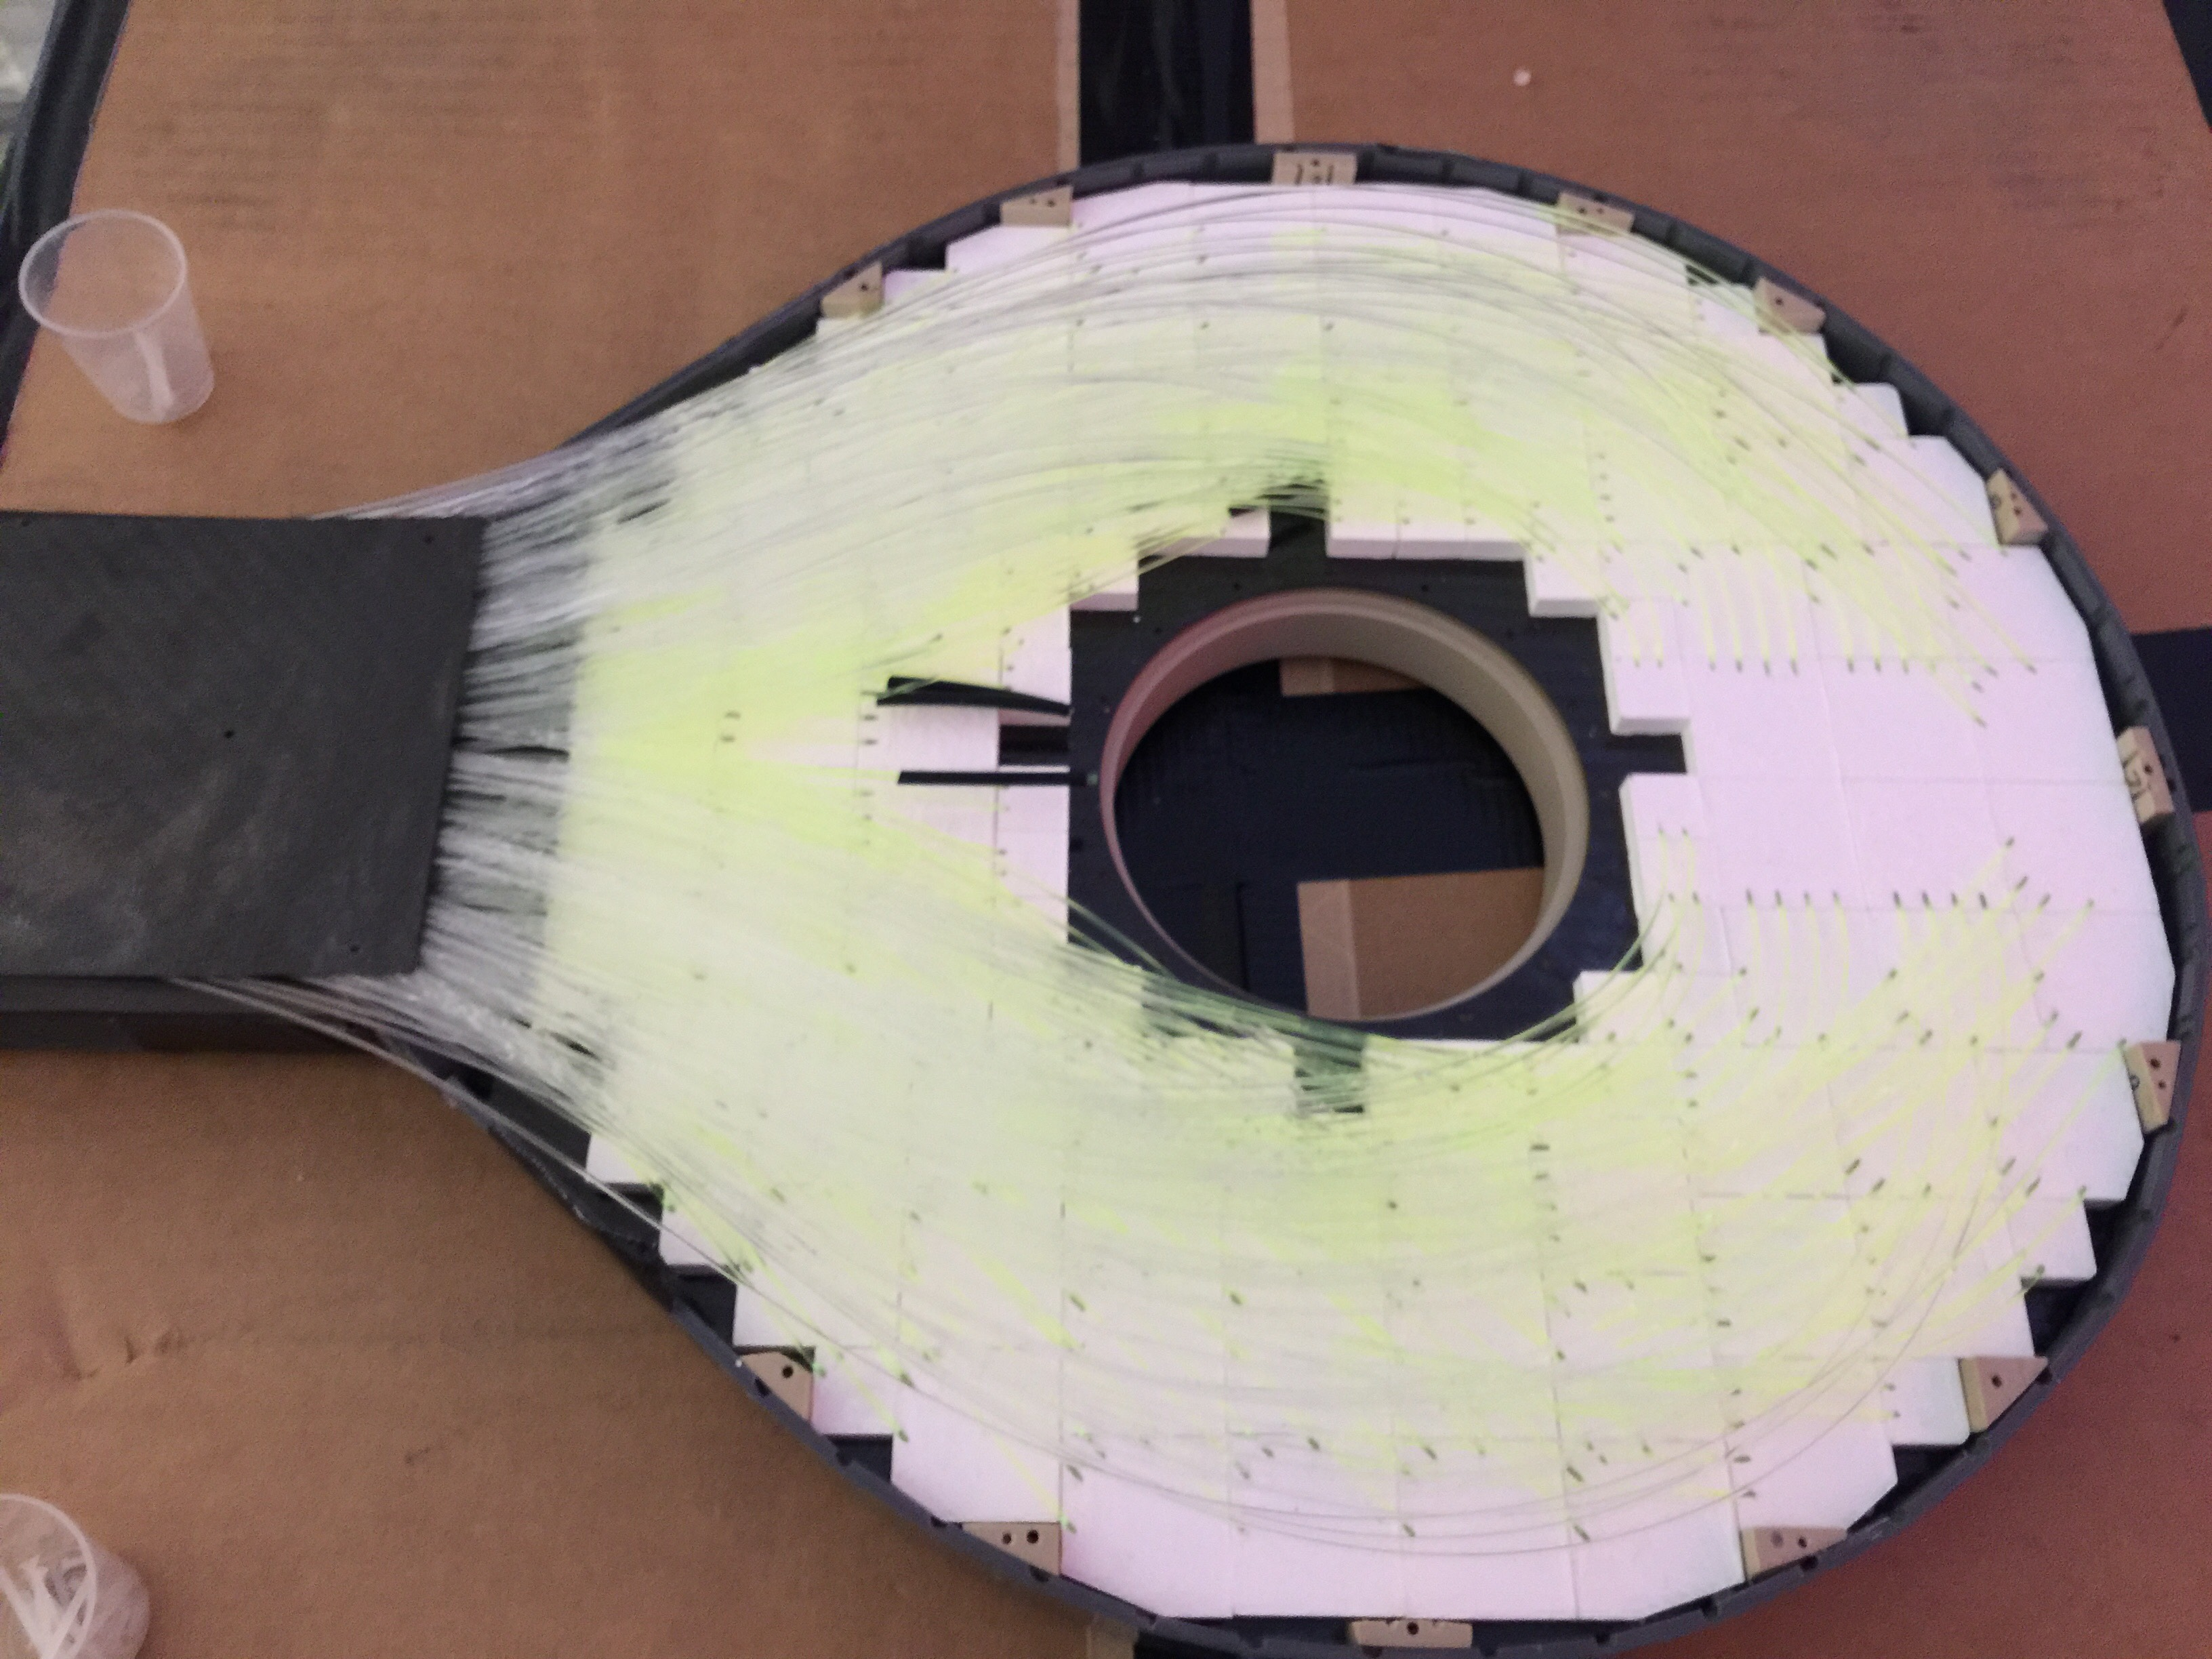
\includegraphics[width=0.6\textwidth]{ImgChap1/hodooverview}
	\caption{A photograph of the hodoscope with the lid from one of the layers removed, exposing the tiles and fibres beneath.}
	\label{hodooverview}
\end{figure}
 
\subsection{Fibre Routing}

After exciting the tiles the fibres are constrained by the limited space available above the tiles across the body of the detector. Ideally each fibre would be allowed to wide smooth curve as possible on its route out of the detector, minimising the light loss due to the curvature of the fibre. However there is limited space available for fibre routing within the detector. Necessitating careful planning to avoid areas of overdensity resricting the fibres exiting tiles, or too much crossover limiting the ammount of fibres that can pass through an area. These constraints are most significant in two areas. First near the bottom of the detector where all the fibres have to pass on their route to the SiPMs. Secondly near the centre of the detector where the density of fibres exciting tiles is highest. 

\begin{figure}
	\centering
	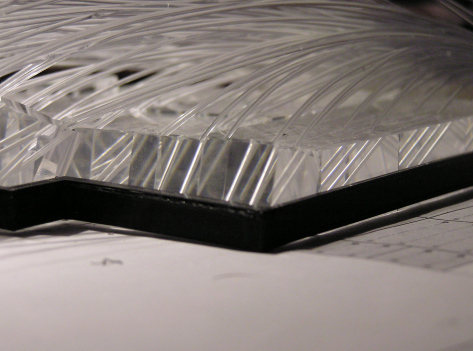
\includegraphics[width=0.6\textwidth]{ImgChap1/fibretest}
	\caption{A photograph of a fibre routing test being carried out to optimise pathing within the detector. The test utilised length of clear fibres inserted into plastic tiles.}
	\label{fibreroutingtest}
\end{figure}

\subsection{Detector Enclosure}

The enclosure that supports the detector elements is based around 4  

The base and lid of each layer of the detector is formed by a sheet of 1mm thick black carbon fibre shaped like an elongated disk with a diameter of 330mm, extended towards at the bottom of the detector, shown in Figure \ref{CarbonFibrePlate}. 

\begin{figure}
	\centering
	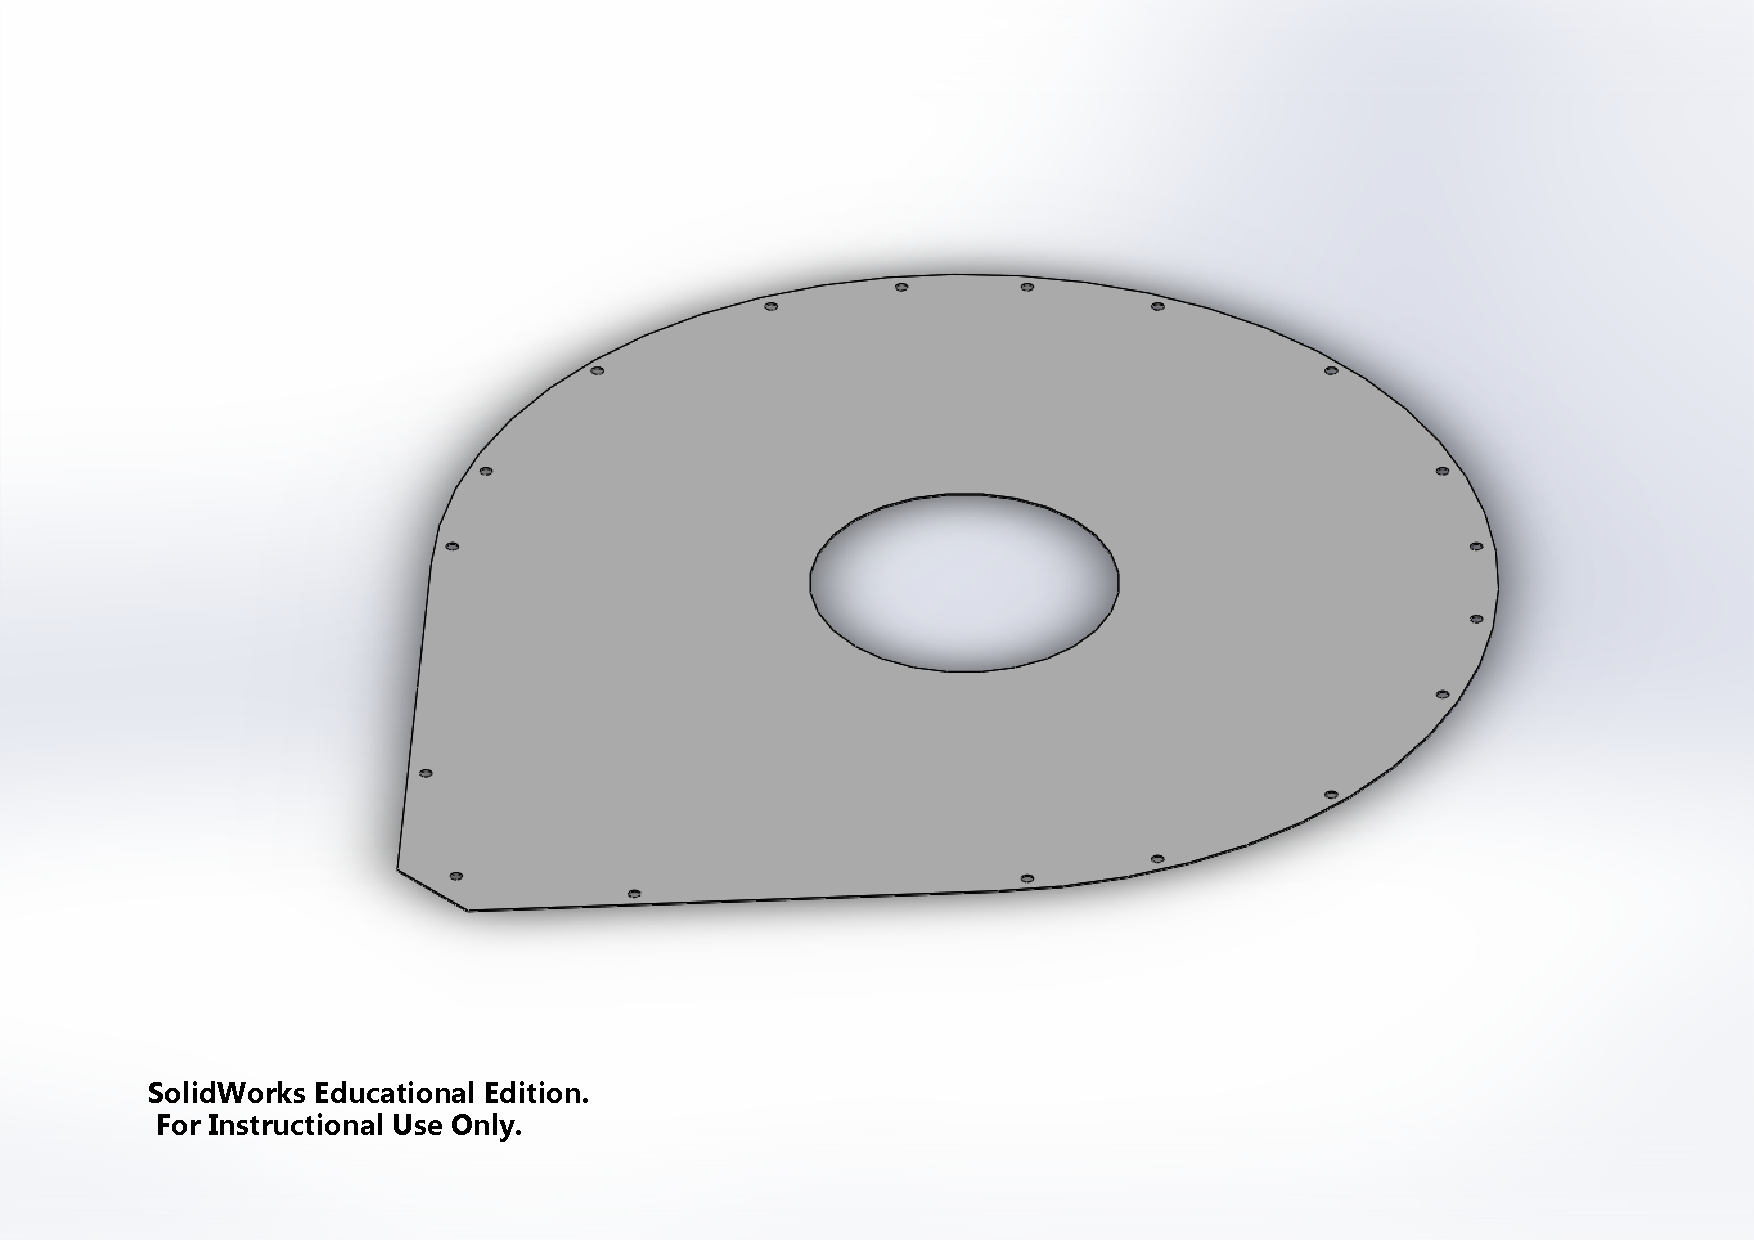
\includegraphics[width=0.6\textwidth]{ImgChap1/CarbonFiberPlateDerek}
	\caption{A CAD diagram of one of the 1mm thick carbon fibre plates used in the hodoscope. \textbf{FIX THE PICTURE}}
	\label{CarbonFibrePlate}
\end{figure}

Between the carbon plates a central \textbf{plastic} support ring and at the outer edge 13 \textbf{plastic} support pillars space the carbon fibre plates, and provide locations for countersunk screws to hold the outer and inner plates in place. Alternate holes pass directly through one layer into the layer below allowing the two layers to helm firmly together by the supporting pillars. The outer pillars are positioned and individually shaped to fill the limited gaps between detector elements and not interfere with the operation of the detector, see Figure \ref{Spacers}.

\begin{figure}
	\centering
	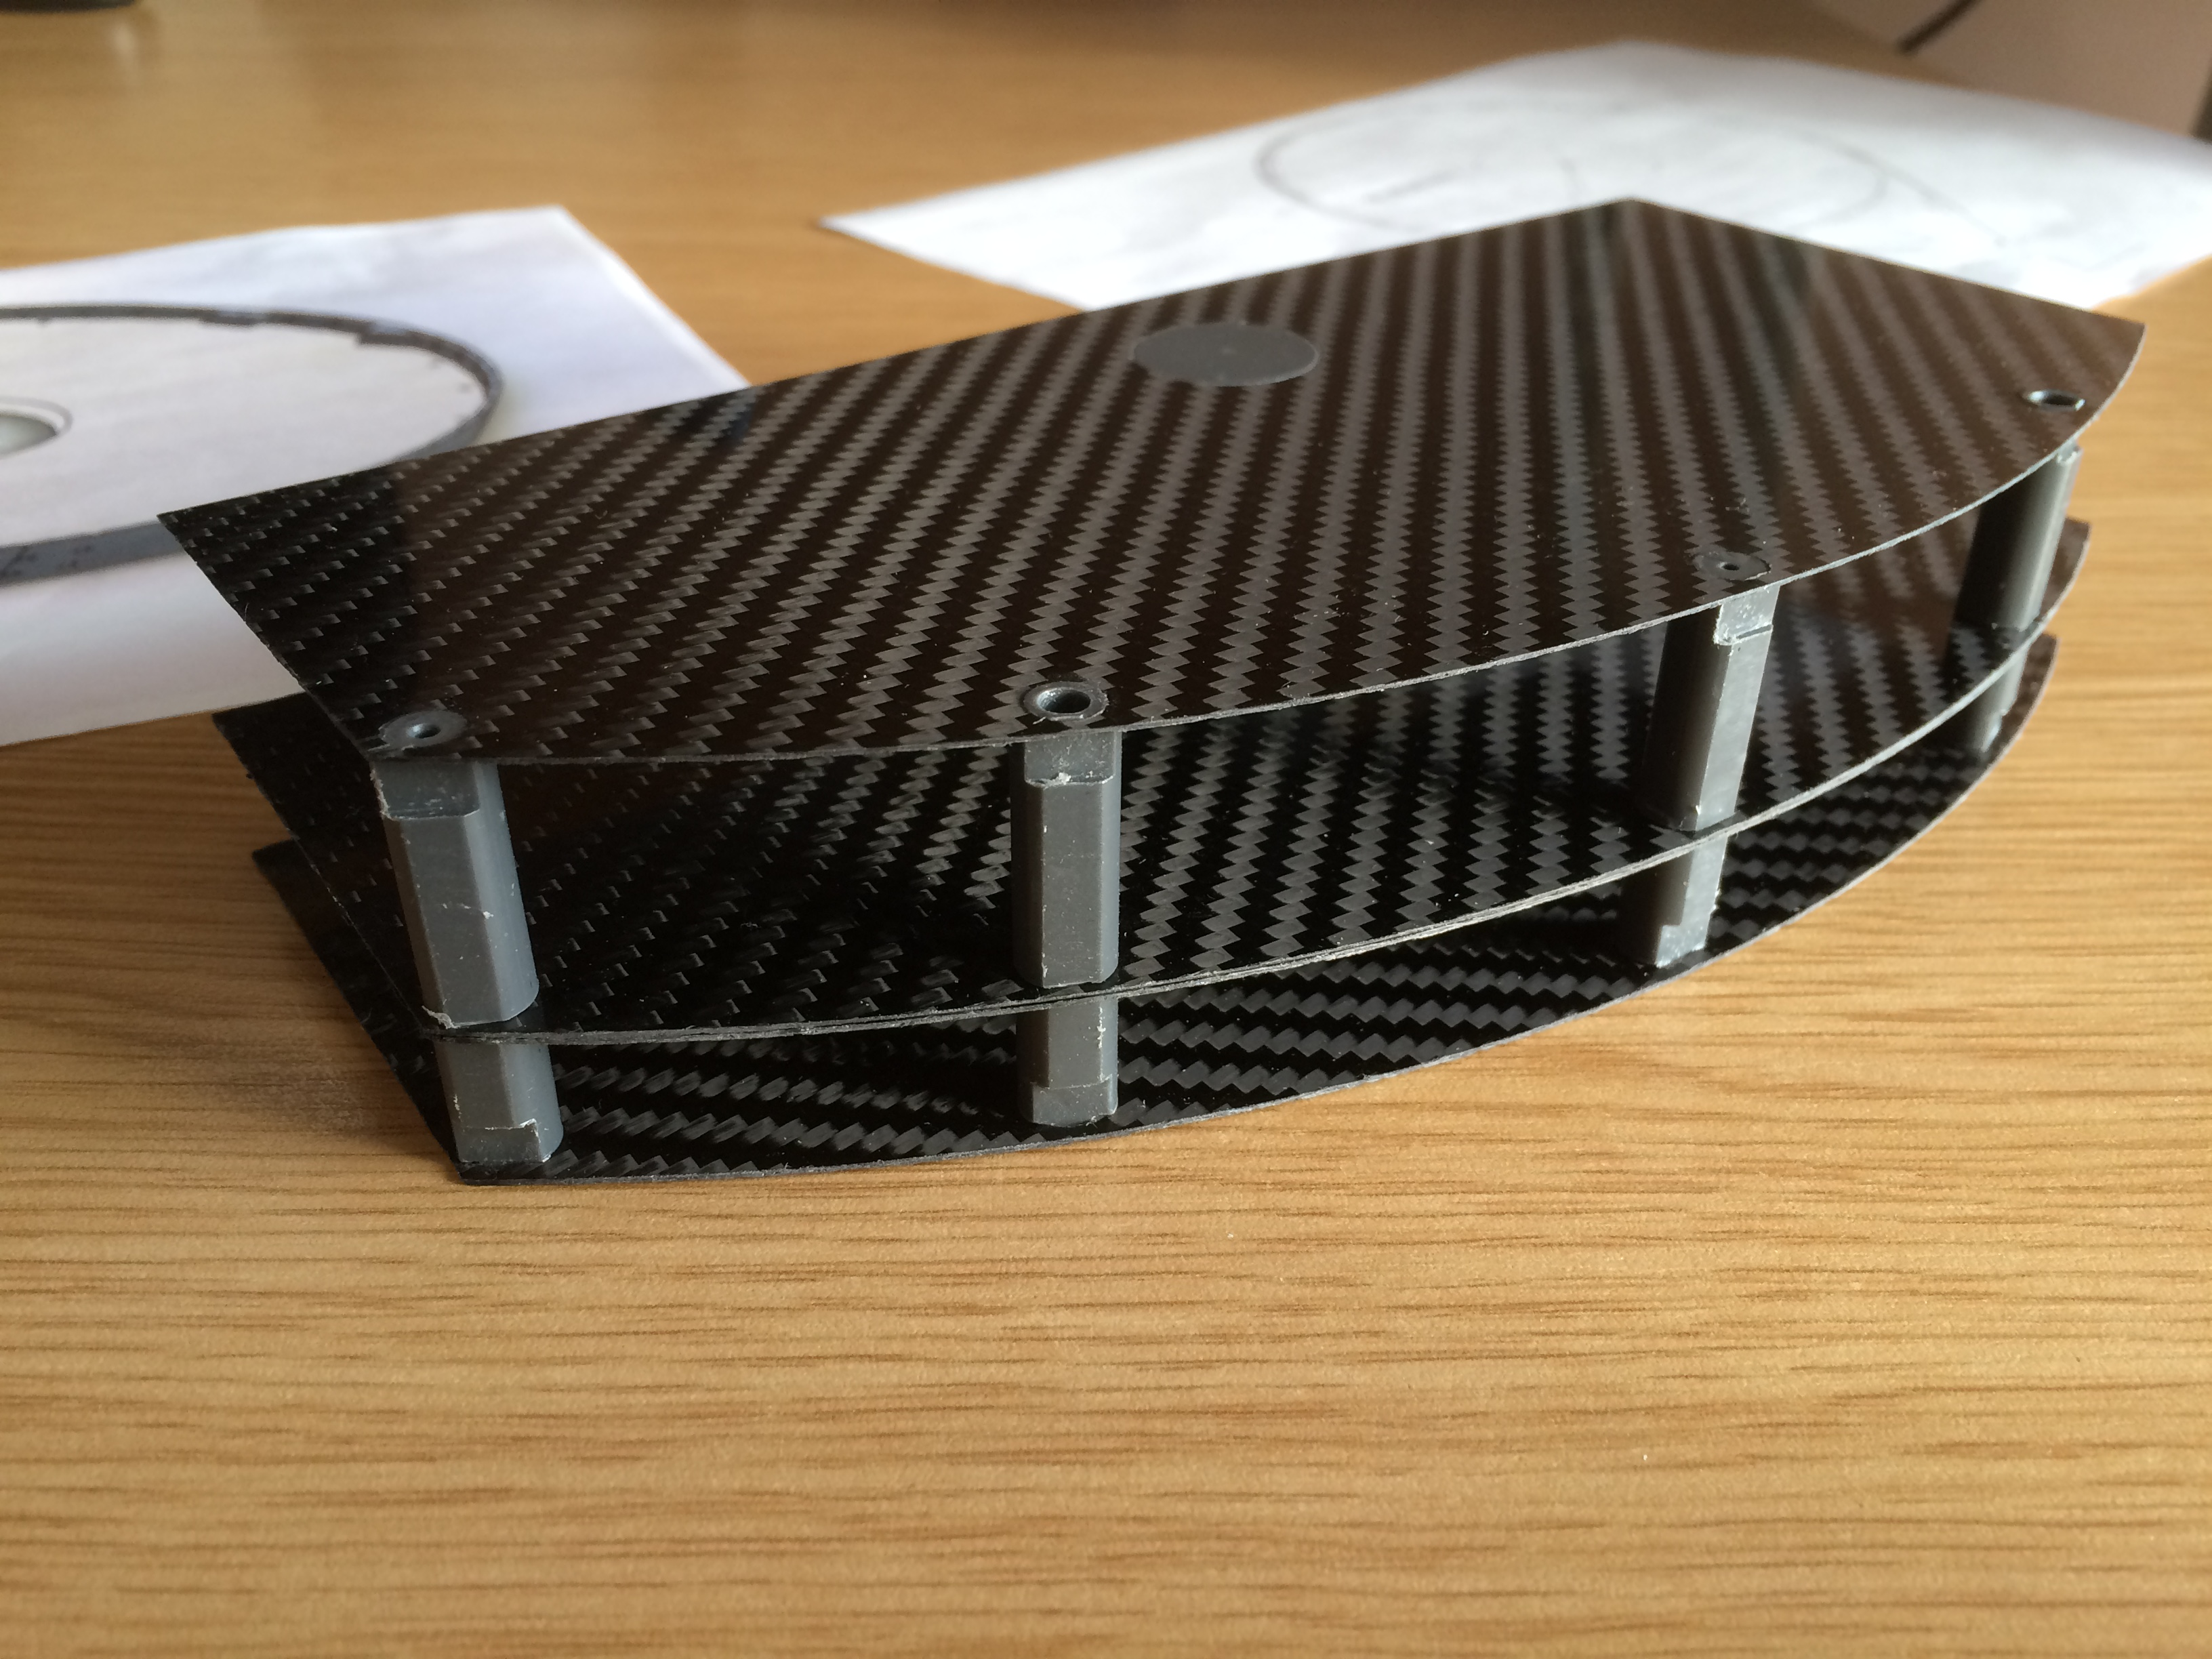
\includegraphics[width=0.6\textwidth]{ImgChap1/enclosure_hodoscope7}
	\caption{A cutaway showing a prototype of the outer spacers used to hold in place and support the carbon fibre disks in the hodoscope.}
	\label{Spacers}
\end{figure}

The fibres in the detector exit each layer through 3D printed component called the delta wing. This critical component acts to channel the fibres out of each layer of the detector, holding them in place and helping to facilitate a light tight seal for the internal components in the detector. It also acts as part of the supporting structure for the detector replacing any supporting pillars at the base of each layer. The fibres are held in place by lacing cords that thread through holes in the base of each side of the delta wing. The component is split into two interlocking pieces, one for each layer of the detector, with greater depth closer to the detector tiles for the layer of thick tiles, before transiting to provide equal square for both sets of fibres along its length. This is shown in Figure \ref{Deltawingsummary}. Just like the main body of the detector, each side of the delta wing is covered by a sheet of 1mm thick carbon fibre secured by countersunk plastic screws, sealing in the fibres it protects. 

\begin{figure}
	\centering
	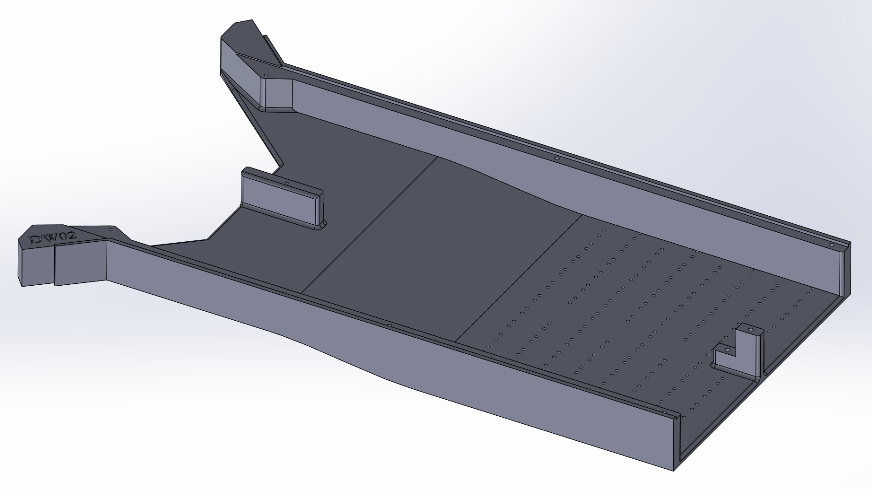
\includegraphics[width=0.6\textwidth]{ImgChap1/deltawingside}
	\caption{A CAD drawing of the hodoscope delta wing section connected to the thin layer of the detector.}
	\label{Deltawingsummary}
\end{figure}

The outer edge of the detector is a flexible plastic strip that bridges the two layers of the detector and is designed to allow the carbon fibre disks to slot seamlessly into channels that run along its length, 2 back to back in the centre and one at the top and bottom, shown in Figure \ref{OuterBelt}. It attaches to the detector system though countersunk screws that fit into the outer pillars of the detector and the delta wing at its base.

\begin{figure}
	\centering
	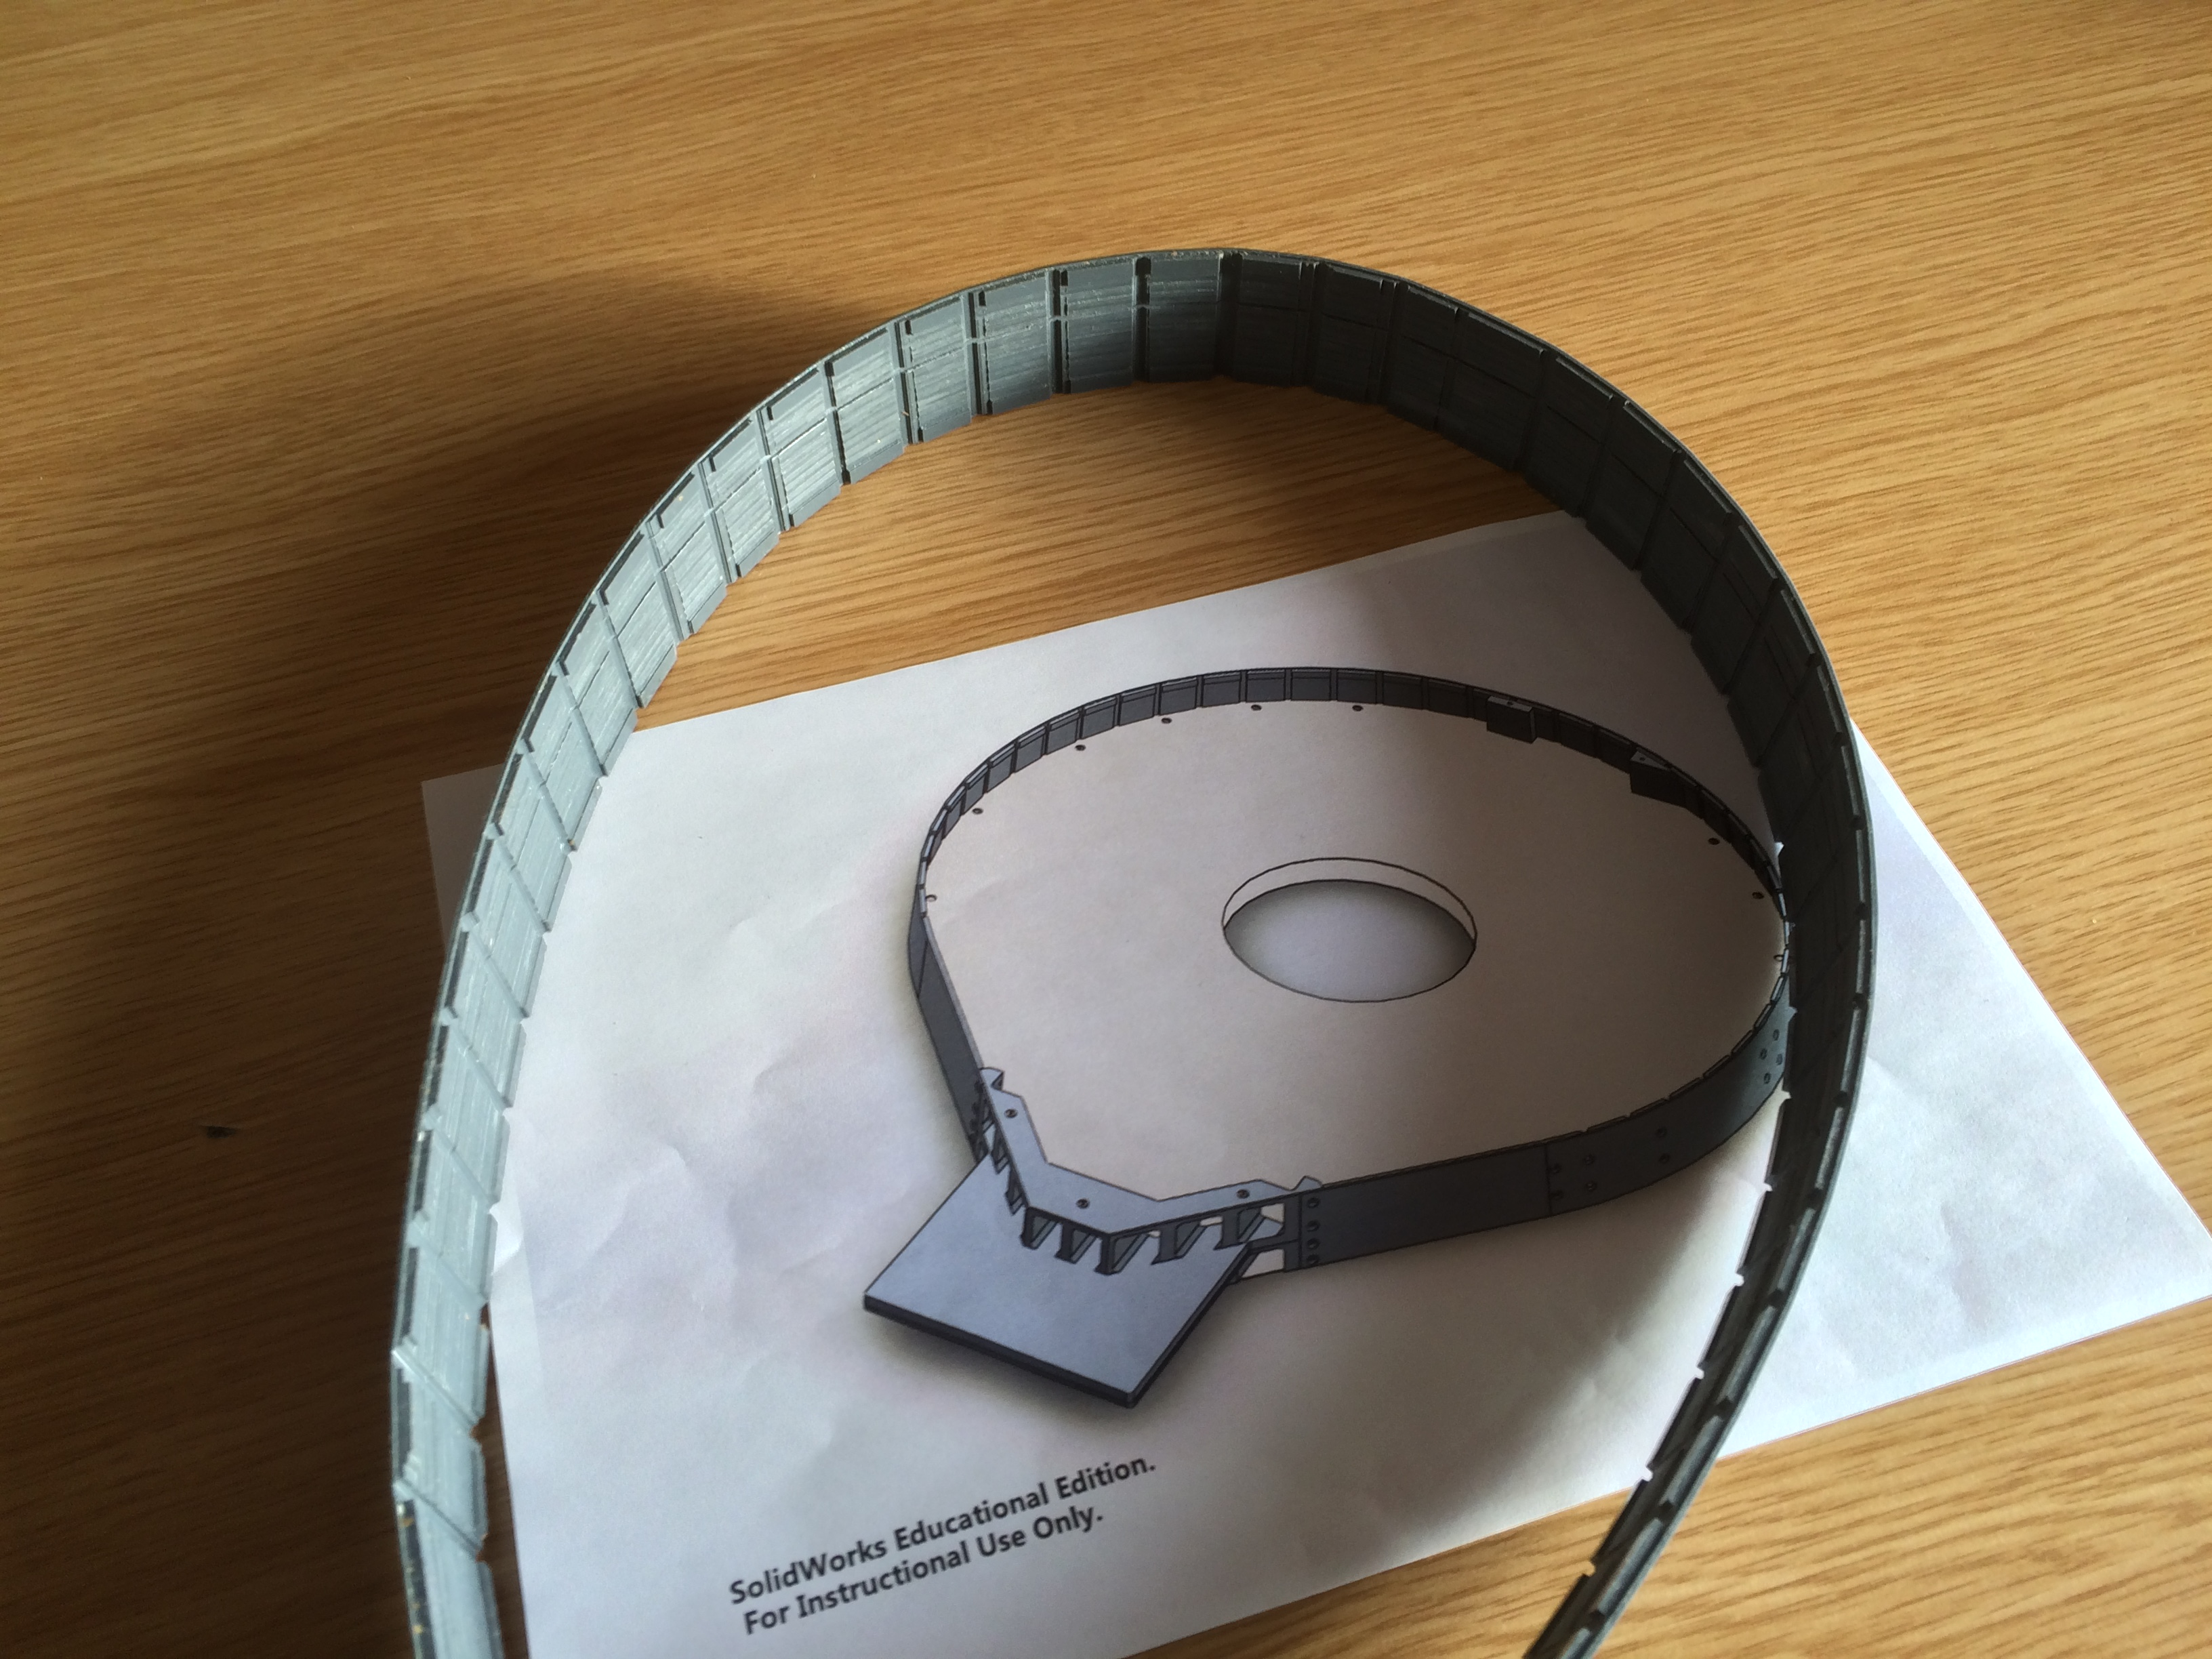
\includegraphics[width=0.6\textwidth]{ImgChap1/enclosure_hodoscope6}
	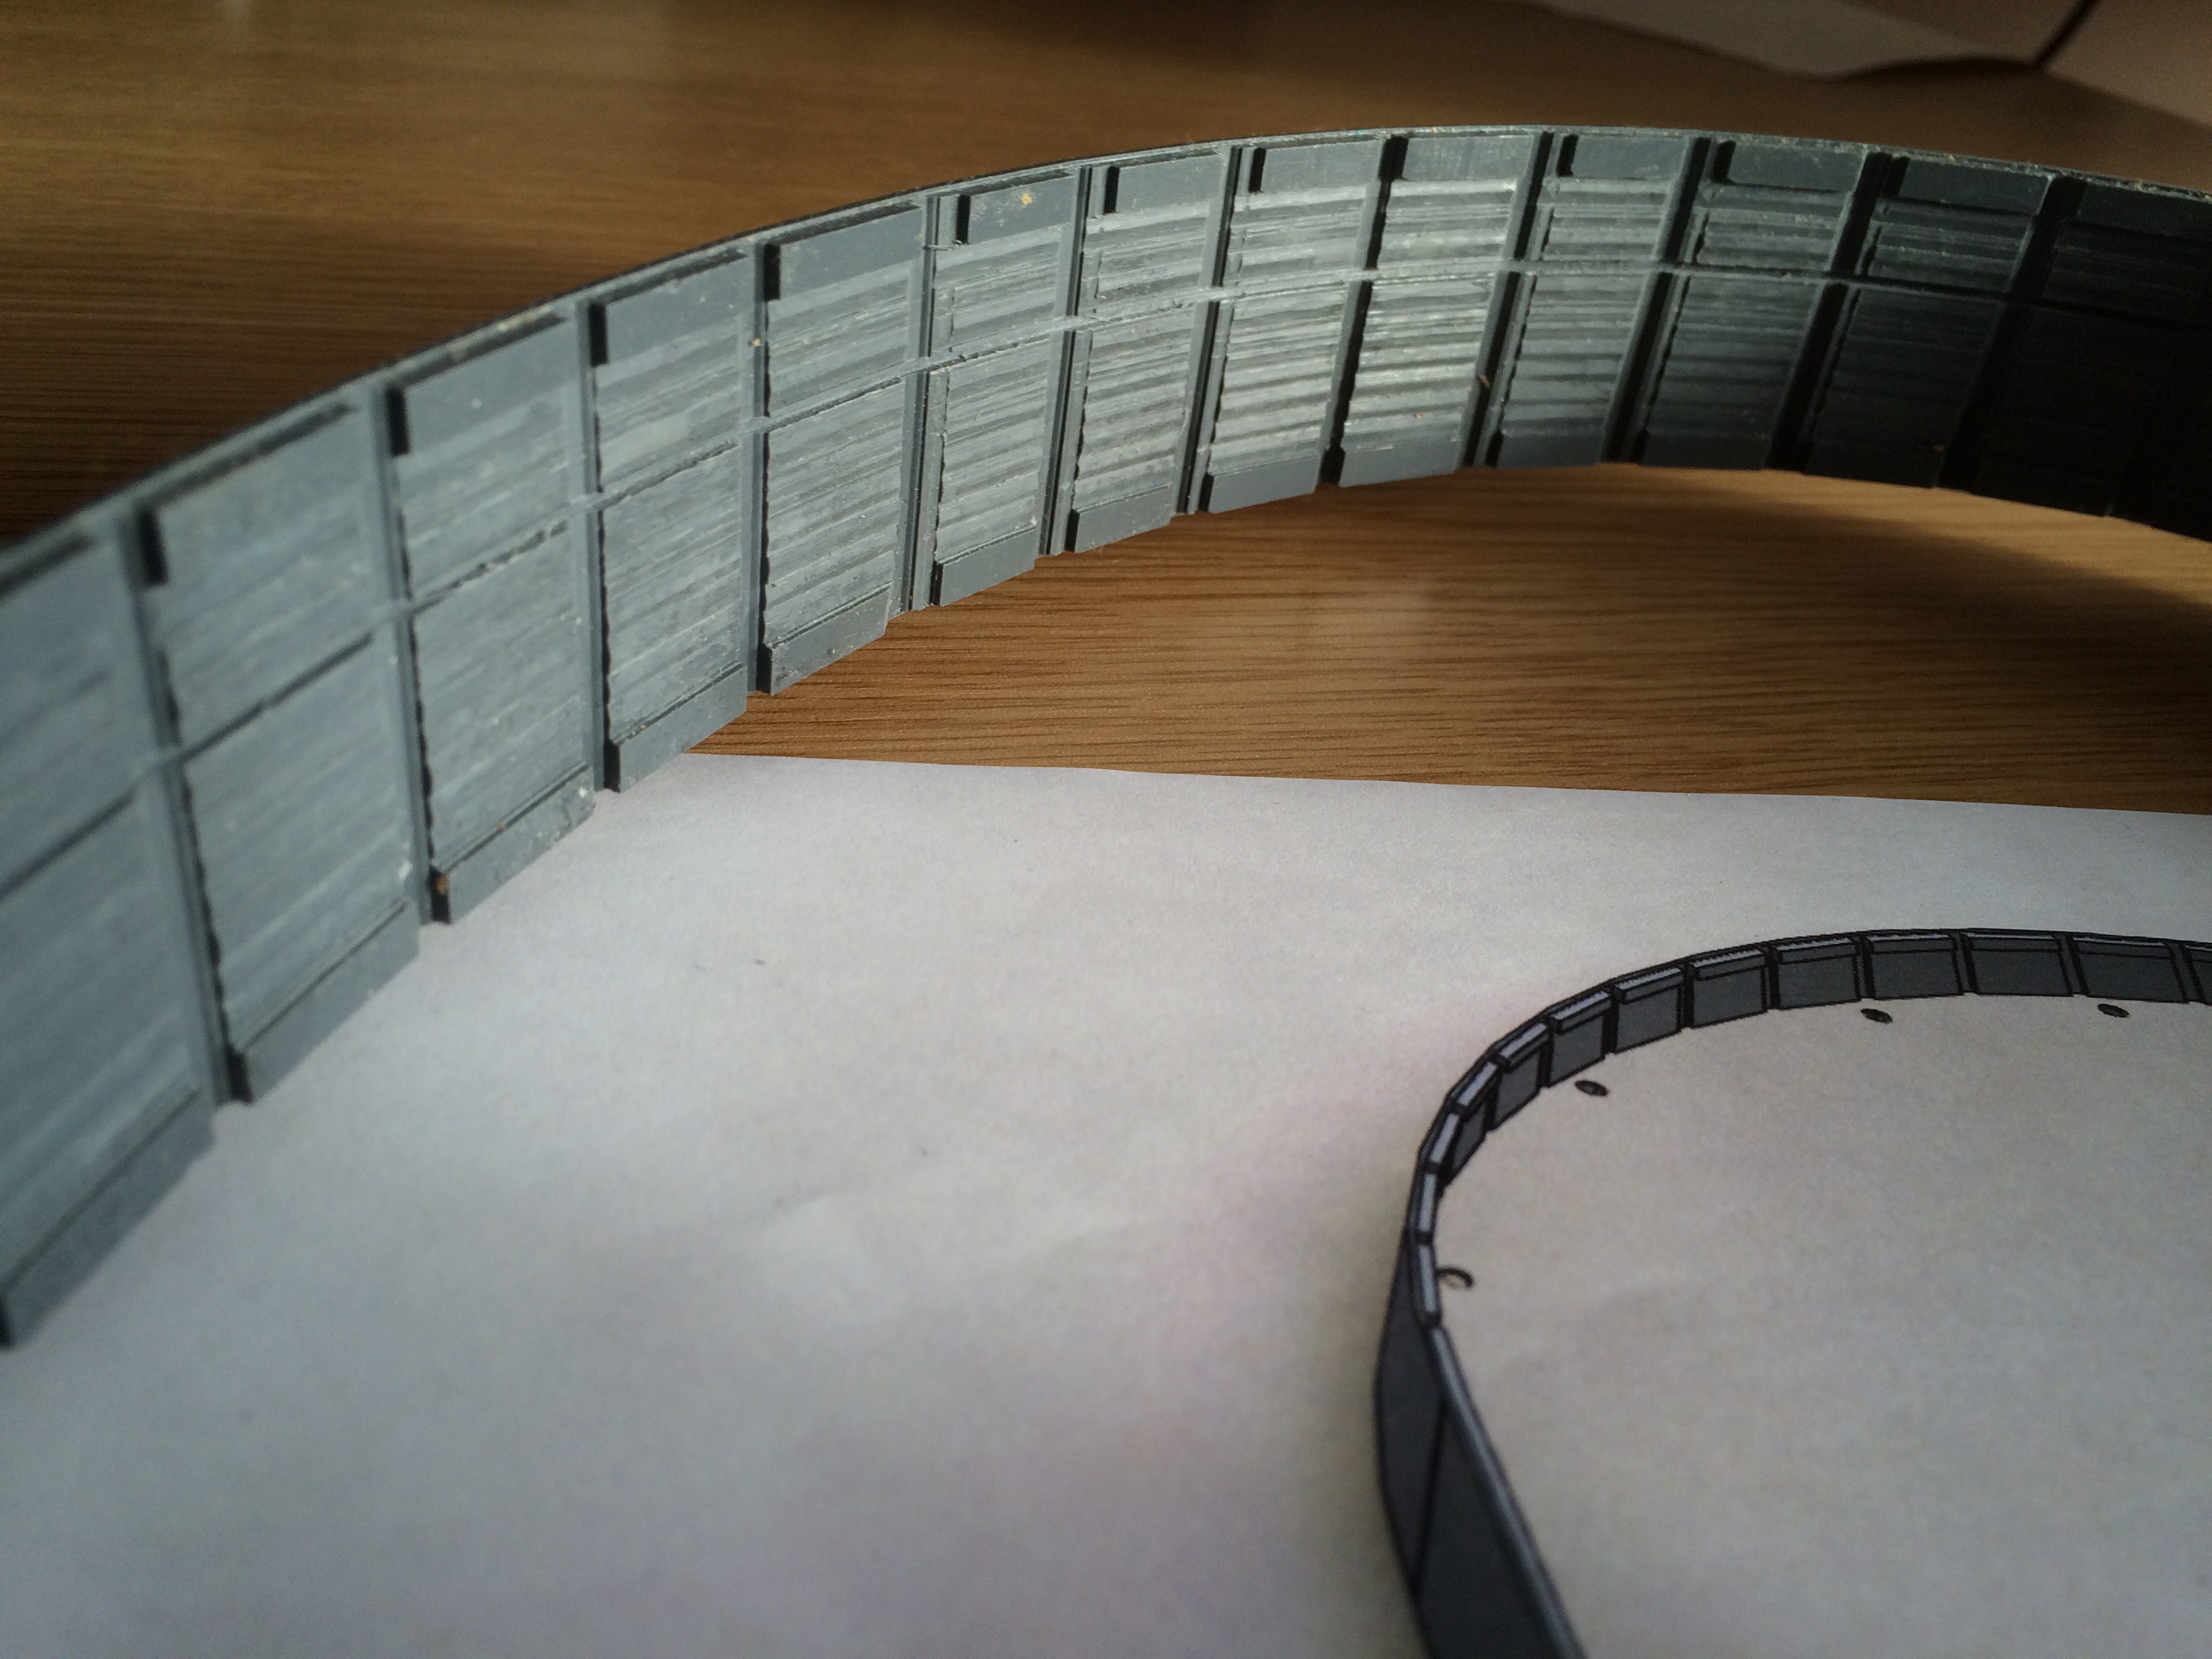
\includegraphics[width=0.6\textwidth]{ImgChap1/enclosure_hodoscope4}
	\caption{Photographs of the flexible plastic strip that forms the outer edge of the hodoscope. The channels for the outer and central carbon fibre disks can be clearly seen. }
	\label{OuterBelt}
\end{figure}

The combination of the pillars and carbon fibre sheets combine to produce a lightweight but rigid and strong construction. The Carbon fibre plates is very strong in the direction of the weave of the carbon fibre, but it is inextensible and brittle in the transverse direction. The pillars, outer rim and delta wing help to offset these issues and the interlocking design spreads any weight bearing accross the entire structure. The structure is also completely composed of materials with low atomic numbers minimising the chance of any rescattering being caused by the detector system.

In between the delta wing connector and the electronics the optical fibres are groups into bundles of 4 that are sealed from light and protected by flexible black PVC sheathing with an internal diameter of 3mm. These are grouped together and pass through CLAS in cables trays, with weight bearing tethers strategically positioned to ensure the weight of the bundles is not bourne by the fibres themselves.


\subsection{Silicon Photomultipliers}

The optical fibres juncture to the SiPMs via a 3D printed 'fishtale' connector which spreads and positions the fibres in ideal locations for optical transmission. Each connector junctions fibres to supply 8 different SiPMs, up to a maximum of 32 optical fibres. The connectors are composed from 3 interlocking pieces, a smoothly widening body, a light sealing lid and end piece into which the fibres are glued, cut and polished. The separate end pieces allow for easier insertion, repairs and replacement of fibres. A CAD drawing of this is shown in Figure \ref{FishtaleDeconstructed}.



\begin{figure}
	\centering
	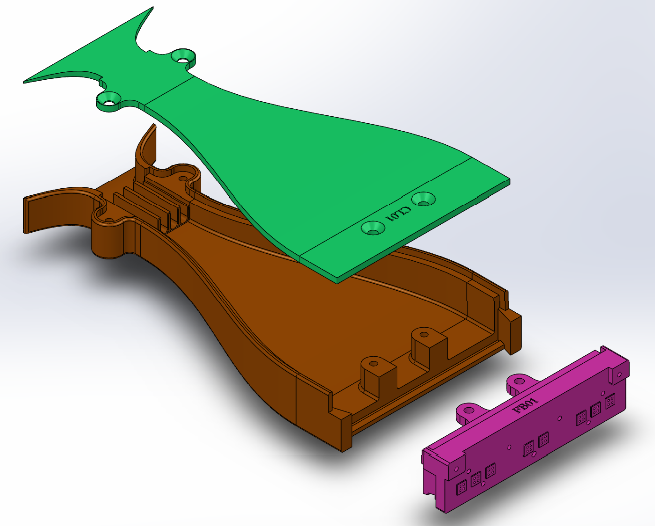
\includegraphics[width=0.5\textwidth]{ImgChap1/fishtail}
	\caption{A deconstructed 'fishtale' connector image showing the different components from which it is formed.}
	\label{FishtaleDeconstructed}
\end{figure}

The fibres from each tile are read out by an individual SiPM. These have high efficiency, high gain, fasting timing response and are sensitive enough to trigger on single photons. These properties make them well suited for a fasting timing detector such as the FT-Hodo. SiPMs are highly sensitive to input voltages requiring high voltage supplies stable to 0.01V for stable operation. However their high gain allows for beautiful clean signal separation from a high energy electron event and their main source of background, thermal noise. With a signal from a thick tile typically 20-30 times the magnitude of the background. To achieve a timing resolution $<0.5ns$ simulations indicated that at least 55 photons to produced by an event need to reach and be accepted by the SiPMs. This is one of the keys goals to surpass when optimising the detectors design and operation. 

The FT-Cal selected APDs over SiPMs because of concerns over possible radiation damage. In the hodoscope they are operating a considerable distance away from the beamline and the main concern, neutron flux, is expected to cause minimal damage over the lifetime of the detector at these distances. \cite{FTTDR2012}.

\begin{figure}
	\centering
	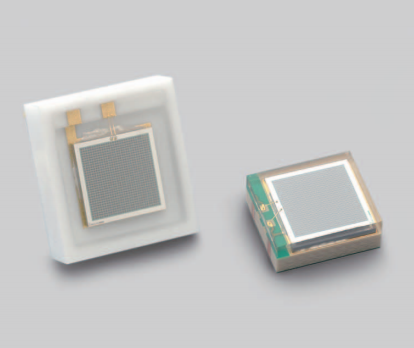
\includegraphics[width=0.5\textwidth]{ImgChap1/sipm}
	\caption{Photograph of 2 3x3mm SiPMs, the right hand model is a surface mounted version that was used in the hodoscope.}
	\label{sipm}
\end{figure}

\subsection{Electronic Boards.}

The SiPMs are mounted mezzanine boards in two groups of 8 with each group supplied by a separate high voltage connection and its own channel by channel adjustable preamplifier boards. There are 15 mezzanine boards in total providing support for the 232 channels of the hodoscope. The all fit into a VME crate along with a control board, with a single low voltage rail supplying PCBs. Through the controller the operation and temperatures of critical components on the boards can be monitored and the high voltage of individual channels adjusted. The SiPMs are gain matched into groups with similar voltage requirements, but adjusting individual channels is necessary for optimal performance. A photo of the front face of the mezzanine boards where the SiPMs are mounted is shown in Figure \ref{electronboards}.

\begin{figure}
	\centering
	\includegraphics[width=0.5\textwidth]{ImgChap1/mezzboards}
	\caption{Photograph of the front face of the mezzanine boards secured in place in the VME crate.}
	\label{electronboards}
\end{figure}

Signals from the amplifier boards are passed to Flash ADCs for processing. \textbf{NEED TO ADD MORE.}

\begin{figure}
	\centering
	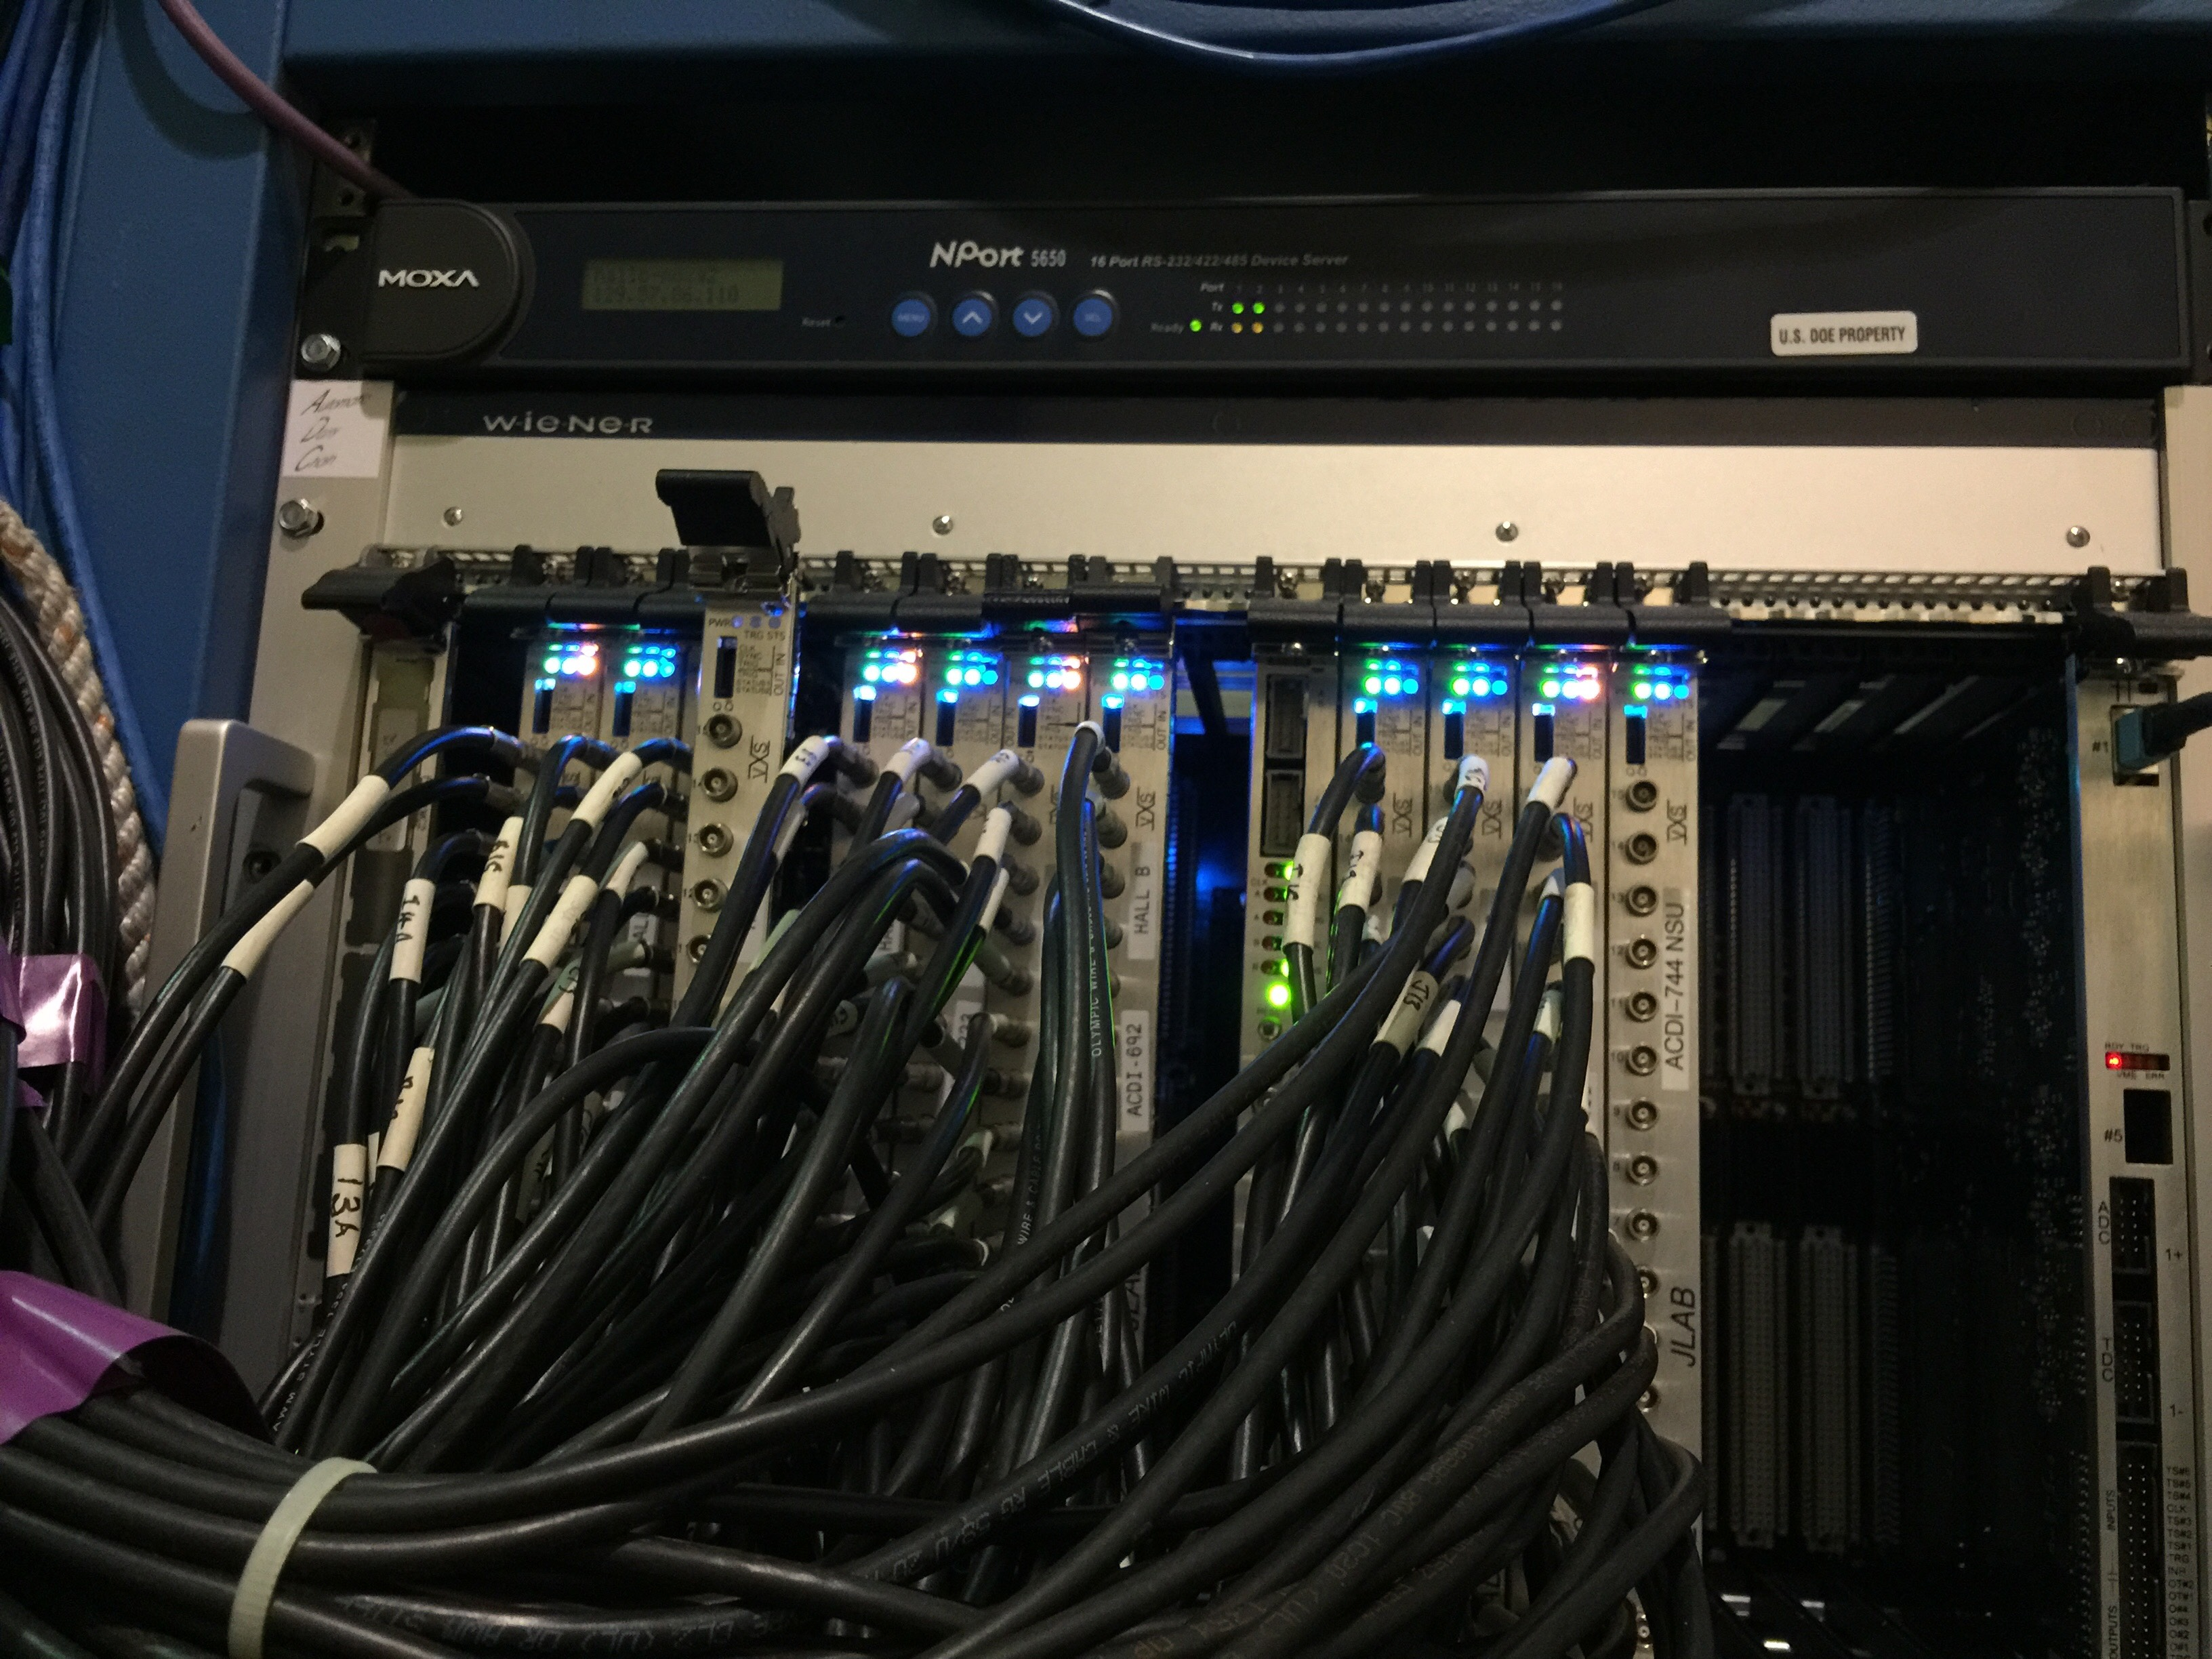
\includegraphics[width=0.5\textwidth]{ImgChap1/FlashADC}
	\caption{Photograph of some of the flashADCs used as read-out from the hodoscope during testing at Jefferson Lab.}
	\label{FlashADC}
\end{figure}

%To achieve this a highly segmented design based on fast responding plastic scintillator tiles   
%
%Describe in more detail the aims and constaints of major design decision of the hodoscope.
%
%Explain decision on choices of tiles, fibres, SiPM etc. Why not other options?
%
%Overall description of the detector



\subsection{Signal Transmission}

For optimal performance of the detector system it is critical to maximise the percentage of photons produced in the scintillators that reach the SiPMs. Improving the capture cross section and transmission of the WLS fibres is essential to this.  Compared to the volume of the scintillators the surface area of the WLS fibres is small and even if a photon enter this region there is a limited photon capture angle for transmission. To improve the chances of capture, each of the tiles is coated in 3 layers of highly reflective $TiO_{2}$ based scintillator paint with a reflectivity of $\sim 96\%$ in photon wavelength range produced by the tiles. Ensuring many passes of the photons are possible before entering the fibres. The ends of the fibres are mirrored used the same material ensure photons that were captured by the fibre but not in the transmission direction of the fibre are reflected back up the fibre towards the SiPMs. 

\begin{figure}
	\centering
	\includegraphics[width=0.5\textwidth]{ImgChap1/meson2}
	\caption{Images of the painted tiles and fibres.}
	\label{PaintedTilesandFibres}
\end{figure}


$TiO_{2}$ paint was selected for its high reflectivity, consistency and ease of application accross the 232 tiles and 784 fibres. Other candidate materials with theoretically higher reflective indices proved either inconsistent or impractical to apply to the geometry and volume of tiles and fibres.

Another critical component in the final output of light at the SiPMs is transmission of the light both within and between material boundaries. Maximising attenuation length in the materials, minimising air gaps and transitions, while keeping those that exist to occur between materials of similar refractive indices. The the quality and consistency of the application of optical cement used between the tiles and fibres, the fusion splice and the precision junction between the optical fibres and the SiPMs are all are the critical points for transmission.

\subsection{Light sealing}

A signal of great amplitude is of limited use unless outside sources of noise can be minimised. In terms of the light yield the essential componants are sealing of the detector system from outside sources of light and isolating each channel from each channel from each other to minimise crosstalk between elements. The entire detector is designed with these twin considerations in mind. 

The reflective coatings around the detector elements maximise their own transmission while simultaneously minimising possible crosstalk. Similar principles follow for the optical fibres, where bend radii are kept above minimum thresholds to increase transmission and reduce crosstalk. 

Points of intersection between different elements of the detector are such as the fishtale connector lids are designed with recesses to provide secure connections between components but also to maximise the length of light path required to pass through, forces light to reflect from multiple matt black surfaces to enter. Reducing the amount of light that passes through any gap. 

\begin{figure}
	\centering
	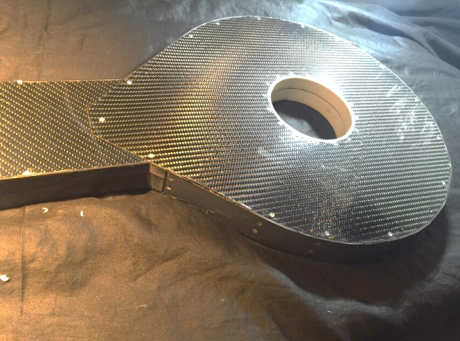
\includegraphics[width=0.7\textwidth]{ImgChap1/sealed}
	\caption{The sealed head of the detector.}		
	\label{sealedlollypop2}
\end{figure}

Most of the surfaces of the detector are made in black for both low transmission and beneficial absorptivity properties. Where possible multiple precautions are engineered into the design of components to minimise the effect of external light sources. For example when groups of fibres pass between the head of the detector and the electronics they are sealed in protective lightproof black PVC sheeting and further sealed by a surrounding layer of tedlar sheeting encompassing all the fibre bundles creating a seamless join between the delta wing of the detector and the entrance to the fishtale connectors. 

%Tedlar sealing.
%
%PVC insulation.
%
%Silicon putty.
%
%Bespoke construction.
%
%Reflective materials.

\subsection{Support structure and Shielding}

Tungsten pipe

Fibre routing through CLAS.

Moeller cone.

\subsection{2 layered design}

Not sure where it's best to insert a section about this.

Thicker layer for increase light output leading to improved timing resolution.

Thinner layer for improved background rejection.

Space limited so a balance between both layers crystal thickness is necessary. Needing to leave space for the support structure and fibres to path out of the detector.